\documentclass[a4paper,12pt,liststotoc,DIV12]{scrartcl}
%\usepackage{geometry}
%\usepackage{ngerman}
\usepackage{longtable}
\usepackage[T1]{fontenc}
\usepackage{ae}
\usepackage[utf8]{inputenc}
\usepackage{fancyhdr}
\usepackage{graphicx}
\usepackage{xspace}
\usepackage[cmyk]{xcolor}
\usepackage{amsmath}
\usepackage[
  %plainpages=false,
  %pdfpagelabels,
  %colorlinks=true,
  pdfborder={0 0 0},
  %urlcolor=blue,
  %linkcolor=blue,
  pdftitle={OST-WeST - Specification},
  pdfsubject={OST-WeST - Specification},
  pdfauthor={Stefan Franke, Robert Hanussek, Benjamin Keil, Steffen Kieß, Johannes Langauf, Christoph Marian Müller, Igor Podolskiy, Tilmann Scheller, Michael Starzmann, Markus Wittlinger},
  pdfkeywords={OST-WeST, Specification},
  bookmarksopen=true,
  %pdfstartpage=3,
  %unicode,
]{hyperref}
% hypcap is needed for correct links to figures, see Bug 2
\usepackage[all]{hypcap} 
\usepackage{svnkw}
\usepackage[USenglish]{isodate}
\usepackage{titlesec}
\usepackage[
  style=altlist,
  number=none,
  hypertoc=true
]{glossary}

% tells glossary package to create a glossary
\makeglossary
\svnid{$Id: Glossary.tex 23 2008-05-28 11:39:25Z ahija $}

\storeglosentry{basic boolean term}{
name={basic boolean term},
description={is the smallest, not further separable part of a boolean expression. Boolean expressions can be separated at their boolean operators leading to smaller boolean expressions and in the end to basic boolean terms. E.g. the Java the \texttt{A ? B : C} operator separates the three boolean expressions A, B and C, which are, if they don't contain further operators, basic boolean terms.}
}

\storeglosentry{basic statement}{
name={basic statement},
description={is a statement, that is not a \gl{looping statement} or a \gl{conditional statement}. For Java the statements \code{return}, \code{throw}, \code{assert} are also excluded.}
}

\storeglosentry{black box test}{
name={black box test},
description={testing the \gl{SUT} with \gl[test case]{test cases} defined on the basis of the functional and non-functional requirements stated in the \gl{specification}.}
}

\storeglosentry{boundary-interior coverage}{
name={boundary-interior coverage},
description={(synonym: C2b) is a type of path coverage. General path coverage is known as incomputable if there are looping statements. To make the problem computable only a limited number of paths are considered. So boundary-interior coverage only examines whether a loop has been executed:
\begin{itemize}
\item never
\item once
\item more than one time
\end{itemize}}
}

\storeglosentry{branch coverage}{
name={branch coverage},
description={(synonym: decision coverage) is a \gl{coverage criterion}. A coverable item is a branch of a \gl{conditional statement}. For branch coverage, a coverable item is covered, if it is entered at least once.}
}

\storeglosentry{CM}{
name={CM},
description={abbreviation for configuration management.}
}

\storeglosentry{code base}{
name={code base},
description={contains all the uninstrumented \gl[code file]{code files} of a specific version of the \gl{SUT}.\\
A code base has a date and time of the first \gl{instrumentation}. If a code base is instrumented from Eclipse, it has a relation to an Eclipse project.}
}

\storeglosentry{code coverage}{
name={code coverage},
description={has two meanings:
\begin{enumerate}
\item is a measurement needed for a \gl{glass box test}. There are different coverage criteria, each defining the \gl[coverable item]{coverable items} and how they are covered.
\item depends on a concrete \gl{coverage criterion} and is defined---only considering the instrumented part of the SUT---as the quotient of the covered coverable items and the total number of coverable items.
\end{enumerate}}
}

\storeglosentry{code file}{
name={code file},
description={is a file containing the whole or a part of the source code of the SUT. For example a \code{*.java} file in Java.}
}

\storeglosentry{condition coverage}{
name={condition coverage},
description={is a \gl{coverage criterion}. Condition coverage defines the \gl[coverable item]{coverable items} as \gl[basic boolean term]{basic boolean terms} used in \gl[statement]{statements} which require a boolean expression that affects the control flow. There are different definitions of when such a basic boolean term is considered as covered---e.g. \gl{strict condition coverage}.}
}

\storeglosentry{conditional statement}{
name={conditional statement},
description={is a \gl{statement} of a specific programming language. Conditional statements are statements creating branches in the control flow, e.g. \texttt{if} or \texttt{switch} in Java. It does not matter, if a \textit{particular} usage of a conditional statement creates a branch (e.g. \texttt{if (true)}) or if branches of a \textit{particular} usage are equal (e.g. \texttt{if (a) \{ \}}). It is a conditional statement creating two branches nonetheless, because an \texttt{if} usually creates two branches.\newline
On the other hand, though the result of some operators depends on a decision, an operator itself creates no branch in the control flow. An example for such an operator would be the \texttt{A ? B : C} operator, of which the result is determined by the value of A. Accounted by itself, such an operator only influences data, not the control flow. Therefore, it is no conditional statement.}
}

\storeglosentry{coverable item}{
name={coverable item},
description={is the smallest unit that can be covered by a coverage criterion, e.g. a \texttt{then} branch in branch coverage.}
}

\storeglosentry{coverage criterion}{
name={coverage criterion},
description={defines the \gl[coverable item]{coverable item} and under which condition they are covered. Some coverage criteria are:
\begin{itemize}
\item \gl{statement coverage}
\item \gl{branch coverage}
\item \gl{condition coverage}
\item \gl{loop coverage}
\end{itemize}}
}

\storeglosentry{coverage log}{
name={coverage log},
description={is a container for raw result data of a coverage run. It contains e.g. counters for all basic statements. This file must be processed afterwards to produce \gl[test session]{test sessions} and \gl[test case]{test cases}.}
}

\storeglosentry{developer}{
name={developer},
description={is a person who is able to write and compile programs in at least one programming language and can understand well documented programs. He is also experienced in both using his computer, especially with file system interaction, web browsing, extracting archive files, applying patches and editing plain text.}
}

\storeglosentry{DocBook XML}{
name={DocBook XML},
description={is a XML based markup language for technical documentation.}
}

\storeglosentry{entry point}{
name={entry point},
description={is the item, that is used to start the \gl{SUT}. For Java, it is a class
file containing the \texttt{main} method. For COBOL, it is the single \gl{code file}.}
}

\storeglosentry{executable file}{
name={executable file},
description={is a compiled code file that can be executed. For Java it is the byte code \code{*.class} file, under COBOL it is a native executable.}
}

\storeglosentry{glass box test}{
name={glass box test},
description={considers the source code of the SUT and aims at reaching a predefined code coverage for a number of coverage criteria.}
}

\storeglosentry{HTML}{
name={HTML},
description={(abbreviation for: Hyper Text Markup Language) is the predominant markup language for the creation of web pages.}
}

\storeglosentry{instrumentable item}{
name={instrumentable item},
description={is an item of the \gl{SUT}. An instrumentable item is a package, containing other instrumentable items, or a code file.}
}

\storeglosentry{instrumentation}{
name={instrumentation},
description={is the process of adding extra code elements to a \gl{code file} in order to get information about the control flow of the running SUT. Instrumentation is used to measure the \gl{code coverage} of the code file.}
}

\storeglosentry{loop coverage}{
name={loop coverage},
description={is a coverage criterion. The loop coverage defines several \gl[coverable item]{coverable items} for each \gl{looping statement}:
\begin{itemize}
\item loop body is not entered
\item loop body is entered once, but not repeated
\item loop body is repeated more than one time
\end{itemize}
Looping statements like do-while cannot be bypassed and have only two possible coverable items.}
}

\storeglosentry{looping statement}{
name={looping statement},
description={is a \gl{statement} of a specific programming language. A looping
statement repeatedly executes a number of statements. For example,
\texttt{for} and \texttt{while} in Java.}
}

\storeglosentry{maintenance engineer}{
name={maintenance engineer},
description={is a \gl{developer} who changes software. He understands technical English. He is able to work out technical details himself, if he is pointed to good documentation.}
}

\storeglosentry{MAST}{
name={MAST},
description={(abbreviation for: More Abstract Syntax Tree) The MAST is a model of the source code containing only the elements of the source code which are necessary to calculate \gl[coverage criterion]{coverage criteria} e.g. \gl[statement]{statements}, branches or boolean expressions which have an affect on control flow.\\
A MAST always refers to a specific \gl{code base}.}
}

\storeglosentry{PDF}{
name={PDF},
description={(abbreviation for: Portable Document Format) is an file format created and controlled by Adobe Systems, for representing two-dimensional documents in a device independent and resolution independent fixed-layout document format.}
}

\storeglosentry{path coverage}{
name={path coverage},
description={is a coverage criterion. To reach full path coverage each of the possible paths from the program entry to the exit must have been followed.}
}

\storeglosentry{project}{
name={project},
description={is an Eclipse project that appears e.g. in the Package Explorer of Eclipse.}
}

\storeglosentry{session container}{
name={session container},
description={is a file in the file system. It contains:
\begin{itemize}
  \item a \gl{code base}
  \item a \gl{MAST} of this code base
  \item a number of \gl[test session]{test sessions} ($\geq$ 0)
\end{itemize}}
}

\storeglosentry{specification}{
name={specification},
description={describes all functional and non-functional requirements the software has to fulfill.}
}

\storeglosentry{statement}{
name={statement},
description={is an element in a \gl{code file} that is the result of the statement production of the grammar of the corresponding programming language.}
}

\storeglosentry{statement coverage}{
name={statement coverage},
description={is a \gl{coverage criterion}. Statement coverage defines the \gl[coverable item]{coverable items} as \gl[basic statement]{basic statements}. A coverable item is covered, if the basic statement is executed. For the Java programming language the execution of the statement has to start to set the statement covered. For COBOL, a basic statement is called covered, if it is executed and the program flow goes to the next statement.}
}

\storeglosentry{strict condition coverage}{
name={strict condition coverage},
description={is a kind of \gl{condition coverage}. Strict condition coverage defines a basic boolean term as covered, if it is evaluated to both true and false and the change from true to false (or false to true) changes the result of the whole condition while every other basic boolean term of the condition remains constant or is not evaluated.}
}

\storeglosentry{SUT}{
name={SUT},
description={(abbreviation for: system under test) The system tested with the software.}
}

\storeglosentry{test case}{
name={test case},
description={
\begin{enumerate}
\item is the description of the input for a test with its expected output according to the \gl{specification}.
\item is an element of a \gl{test session} containing a part or all of the \gl{code coverage} results for code files depending on a set of coverage criteria. Additional information which are stored with a test case are: 
 \begin{itemize}
  \item a name
  \item date and time of measurement
  \item a comment
  \item the related test session
 \end{itemize}
If the test case is related to a JUnit test case or test method extra information are needed:
 \begin{itemize}
  \item the names of the test methods of the JUnit test case
  \item whether the test methods of the JUnit test case failed or not
  \item if a test method failed, which failure respectively error was the reason
 \end{itemize}
\end{enumerate}}
}

\storeglosentry{test session}{
name={test session},
description={is the result of a coverage measurement of the SUT by the software. It has:
\begin{itemize}
  \item a name
  \item a date and a time of measurement
  \item a comment
\end{itemize}
and contains:
\begin{itemize}
  \item a number of \gl[test case]{test cases} ($\geq$ 0)
  \item the measurement results 
  \item calculated coverage by \gl[instrumentable item]{instrumentable item} 
  \item a reference to a \gl{code base}
  \item possibly a reference to a related Eclipse \gl[project]{project}
\end{itemize}}
}
%Usage: \gl{entry} or \gl[entry]{entry in context}
%Example: It is one \gl{test case} but several \gl[test case]{test cases}.
\newcommand{\gl}[2][\undefined]{\ifx#1\undefined%
\useGlosentry[]{#2}{#2}\textsuperscript{\begin{tiny}$\nearrow$\end{tiny}}%
\else\useGlosentry[]{#1}{#2}\textsuperscript{\begin{tiny}$\nearrow$\end{tiny}}\fi}

\makeatletter

% some TeX voodoo to extract the date from SVN ID
% which can be processed by isodate 
\def\svn@dateonly#1 #2Z{#1}
\def\svndateonly#1{%
\ifx#1\empty1970-01-01\else
\expandafter\svn@dateonly#1\fi}

% Two-level figure & table numbering
\@addtoreset{table}{section}
\@addtoreset{figure}{section}
\renewcommand{\thefigure}{\thesection.\arabic{figure}}
\renewcommand{\thetable}{\thesection.\arabic{table}}
\makeatother

% custom font sizes for headings, non run-in titles for [sub]paragraphs
\titleformat{\section}{\bfseries\fontsize{24}{30}\selectfont\sffamily}{\thesection}{1em}{}
\titleformat{\subsection}{\bfseries\fontsize{18}{24}\selectfont\sffamily}{\thesubsection}{1em}{}
\titleformat{\subsubsection}{\bfseries\fontsize{16}{22}\selectfont\sffamily}{\thesubsubsection}{1em}{}
\titleformat{\paragraph}{\bfseries\fontsize{14}{20}\selectfont\sffamily}{\theparagraph}{1em}{}
\titleformat{\subparagraph}{\bfseries\normalsize\sffamily}{\thesubparagraph}{1em}{}
\titlespacing{\paragraph}{0pt}{\parskip}{-0.5\parskip}{}
\titlespacing{\subparagraph}{0pt}{\parskip}{-0.5\parskip}{}

\svnid{$Id: Specification.tex 1 2007-12-12 17:37:26Z t-scheller $}

\parindent0mm
\parskip2mm
%\geometry{textwidth=160mm, textheight=230mm, inner=30mm}

\xdefinecolor{TodoColor}{rgb}{1.0, 0.0, 0.0}
\xdefinecolor{JUnitFailure}{rgb}{0.27, 0.4, 0.57}
\xdefinecolor{JUnitError}{rgb}{0.87, 0.12, 0.18}

% depth of the headlines that are numbered
\setcounter{secnumdepth}{5}
\setcounter{tocdepth}{2}

\newcommand{\OSTWeST}{\textit{OSTWeST}\xspace}
\newcommand{\gbt}{\textit{CodeCover}\xspace}
\newcommand{\eclui}{\textsc}
\newcommand{\code}{\texttt}
\newcommand{\todo}[1]{\bgroup\color{TodoColor}\textsc{\textbf{TODO:} #1}\egroup}
\newcommand{\BIG}{\fontsize{48}{48}\selectfont}
%% usage \linkwithfootnote{http://junit.org}{JUnit}
\newcommand{\linkwithfootnote}[2]{\href{#1}{#2}\footnote{\url{#1}}}

% needed for the Function Point tables
\newcommand{\x}{\textbullet}

\includeonly{VersionHistory,Introduction,UserInterface,FunctionalRequirements,NonFunctionalRequirements,Glossary}
%\includeonly{Introduction}
%\includeonly{UserInterface}
%\includeonly{FunctionalRequirements}
%\includeonly{NonFunctionalRequirements}
\begin{document}

% --- title page --- %
\pagestyle{empty}
\begin{titlepage}
 \vspace*{38mm}
 \begin{center}
 \fontsize{24}{24}\selectfont
 Specification\\
 \vspace*{12mm}
 \fontsize{48}{48}\selectfont
 
 % gross hack to generate the a big fancy gbt-squared appearance
 \textit{CodeCover}
 %
 \\
 \fontfamily{\familydefault}\fontsize{32}{38}\selectfont
 Glass Box Testing Tool\\
 \vspace*{12mm}
 \fontsize{16}{20}\selectfont
 Student Project A ``OST-WeST''\\
 University of Stuttgart

 \vspace{2cm}
 {\small 
   Version: 1.1-dev \\
   {Last changed on \printdate{\svndateonly{\svndate}} (SVN Revision \svnrev)}}
   \end{center}
   \vspace{3cm}
   \hspace{40mm}
   \normalsize
\end{titlepage}

% --- Header and version history --- %

\cleardoublepage
\fancyhf{}
\fancyhead[RE,LO]{\textit{\gbt - Specification}}
\fancyhead[RO,LE]{\thepage}
\pagestyle{fancyplain}

% -- Version History -- %
\svnid{$Id: VersionHistory.tex 23 2008-05-28 11:39:25Z ahija $}

\section*{Version History}

{\small
\begin{longtable}{|l|l|p{35mm}|p{71mm}|} \hline
   {\normalsize \textbf{Date}} &
   {\normalsize \textbf{Version}} &
   {\normalsize \textbf{Author}} & 
   {\normalsize \textbf{Modifications}} \\\hline \hline \endhead
    11.01.2007 &  0.1 &  Stefan Franke & 
      - Chapter files and master document file \\\hline
    16.01.2007 &  0.2 &  Stefan Franke & 
      - ui: Eclipse Plug-in and images within \\\hline
    17.01.2007 &  0.3 & Michael Starzmann \newline Christoph Müller & 
      - Headwords following the corresponding chapter in the analysis-notes \newline
      - nr: Keywords taken over by the analysis notes \newline
      - fr: The foreword for the functional requirements \\\hline
    18.01.2007 &  0.4 &  Stefan Franke & 
      - ui: Rewrite source code highlighting \newline
      - Reorder chapters \newline
      - Rename some sections \newline
      - ui: Added source code highlighting for COBOL \\\hline
    19.01.2007 &  0.5 &  Christoph Müller & 
      - Document structure changed \newline
      - fr: Use case pictures imported \newline
      - fr: Foreword, fr: actors, fr: general arrangements \\\hline
    20.01.2007 & 0.6 & Johannes Langauf \newline Christoph Müller & 
      - nf: Expand some keywords to complete sentences \newline
      - nf: Find new NFRs \newline
      - fr: Configuration \newline
      - fr: Use case description \newline
      - fr: Language support \\\hline
    21.01.2007 & 0.7 & Christoph Müller \newline Stefan Franke & 
      - fr: Use case description \newline
      - ui: Session view, Coverage view and Launching \\\hline
    23.01.2007 & 0.8 & Christoph Müller \newline Stefan Franke \newline Michael Starzmann& 
      - Correction after specification meeting \newline
      - fr: Use case description of measure coverage \newline
      - fr: General functional requirements \newline
      - fr: Reports \newline
      - ui: Configuration dialogs \\\hline
    24.01.2007 & 0.9 & Michael Starzmann \newline Christoph Müller & 
      - in: Introduction \newline
      - fr: Use case description \newline
      - fr: Coverage Criteria \\\hline
    25.01.2007 & 0.10 & Michael Starzmann \newline Stefan Franke & 
      - ui: Package and file selection to ... states \newline
      - fr: Coverage measurement improved \newline
      - in: Introduction \\\hline
    26.01.2007 & 0.11 & Christoph Müller \newline Stefan Franke & 
      - Correction after specification meeting \newline
      - fr: New use case instrument instrumentable items \newline
      - ui: Configuration sections \newline
      - ui: Source code highlighting \\\hline
    27.01.2007 & 0.12 & Christoph Müller \newline Stefan Franke \newline Michael Starzmann & 
      - fr: Use case description of administrate sessions \newline
      - ui: Instrumentation subsection \newline
      - ui: Solved todos \newline
      - ui: first draft for the Batch interface \newline
      - fr: Release, folders, files \\\hline
    28.01.2007 & 0.13 & Christoph Müller \newline Stefan Franke \newline Johannes Langauf & 
      - fr: Batch interface \newline
      - ui,fr: Correction after internal review \newline
      - nr: improve and fill out most non-functional requirements \\\hline
    29.01.2007 & 0.14 & Christoph Müller & 
      - fr: Solve todos, use case diagrams, folder structure \newline
      - Correction after QA meeting \newline
      - small spell check \\\hline
    30.01.2007 & 0.15 & Christoph Müller \newline Stefan Franke \newline Johannes Langauf & 
      - fr: New use cases: analyse coverage log, export session \newline
      - ui: New Context menu \newline
      - ui: Import, Export, Report \newline
      - ui: Small adaption at figures \newline
      - nf: Correction after specification review \newline
      - nf: Extensibility, performance requirements, program examples \\\hline
    31.01.2007 & 0.16 & Christoph Müller \newline & 
      - Correction after Igor's big bang \\\hline
    31.01.2007 & 1.0 & Igor Podolskiy & Declaring version 1.0, ready for review \\\hline
    08.02.2007 & 1.1-dev-1 & Stefan Franke \newline Michael Starzmann & 
      - Correction after specification review \\\hline
    09.02.2007 & 1.1-dev-2 & Christoph Müller & 
      - Correction after specification review \\\hline
    10.02.2007 & 1.1-dev-3 & Christoph Müller & 
      - Correction after specification review: Bugs 47, 90, 52, 57, 56, 58, 60, 62, 63, 64, 65, 39, 40, 41, 42, 44, 46, 50, 51, 52, 54, 34 \\\hline
    11.02.2007 & 1.1-dev-4 & Johannes Langauf \newline Christoph Müller \newline Stefan Franke & 
      - Correction after specification review: Bugs 48, 35, 32, 91, 16 \\\hline
    12.02.2007 & 1.1-dev-5 & Johannes Langauf \newline Christoph Müller  &
      - Correction after specification review: Bug 22 \newline
      - new batch commands \\\hline
    13.02.2007 & 1.1-dev-6 & Stefan Franke \newline Christoph Müller &
      - moved the glossary to specification document \newline
      - added links to glossary entries \newline
      - Bug 7: Work flow \newline
      - Bugs 6, 21, 28, 88, 89, 91\\\hline
    14.02.2007 & 1.1-dev-7 & Stefan Franke \newline Christoph Müller \newline Michael Starzmann &
      - Bug 45 \\\hline
    16.02.2007 & 1.1-dev-8 & Stefan Franke \newline Christoph Müller &
      - Bug 45 \\\hline
    11.05.2007 & 1.1-dev-9 & Stefan Franke \newline Christoph Müller &
      - Bugs 98, 99, 100 \\\hline
    15.06.2007 & 1.1-dev-10 & Christoph Müller & 
      - fr: \ref{fr:JUnit integration} JUnit integration \\\hline
    17.06.2007 & 1.1-dev-11 & Stefan Franke & 
      - ui: \ref{ui:Boolean Analyzer} Boolean Analyzer \\\hline
    18.06.2007 & 1.1-dev-12 & Christoph Müller & 
      - fr: \ref{fr: Coverage measurement} coverage log file name \newline
      - fr: \ref{fr:Batch:Instrument} instrument supports a charset  \newline
      - fr: \ref{fr:Batch:Analyze} analyze supports a charset \newline
      - fr: \ref{fr:Batch:Instrumenter-info} Instrumenter-info \\\hline
    19.06.2007 & 1.1-dev-13 & Christoph Müller & 
      - fr: \ref{fr:Batch:Instrument} instrument has \verb$--$copy-uninstrumented \\\hline
    29.06.2007 & 1.1-dev-14 & Christoph Müller & 
      - fr: \ref{fr:Batch:Instrument} instrument has include, exclude \\\hline
    19.09.2007 & 1.1-dev-15 & Johannes Langauf & 
      - ui: \ref{ui:Hot-Path} Hot-Path: make outstanding decisions, update for configureable colors \newline
      - fr: remove PDF-Report support \\\hline
     31.10.2007 & 1.1-dev-16  & Tilmann Scheller  & general update of specification
       \\\hline
    28.05.2008 & 1.1-dev-17 & Christoph Müller & 
      - fr: \code{return} and \code{break} are basic statements too \\\hline
%     &   &   & 
%       \\\hline
\end{longtable}
}

%%% Local Variables: 
%%% mode: latex
%%% TeX-PDF-mode: t
%%% TeX-master: "Specification.ltx"
%%% End: 


% \cleardoublepage

% --- Table of contents --- %

\parskip1mm
\tableofcontents
\parskip2mm

\pagestyle{fancyplain}
\renewcommand{\baselinestretch}{1.25}\normalsize

\svnid{$Id: Introduction.tex 1 2007-12-12 17:37:26Z t-scheller $}
\section{Introduction} \label{Introduction}

\subsection{Project overview} \label{in:Overview}
\gbt stands for \textbf{g}lass \textbf{b}ox \textbf{t}esting \textbf{t}ool. It measures the \gl[code coverage]{code coverage} of a running program and will be as independent as possible of the programming language of the covered program.
\par
Characteristics of \gbt:
\begin{itemize}
  \item \gbt runs at least on Linux and Windows,
  \item \gbt can measure code coverage for programs written in Java and COBOL.
  \item \gbt is extensible to measure code coverage for further programming languages as well.
  \item \gbt measures multiple code coverage criteria and is extensible to further ones.
  \item \gbt provides functionality to create reports of the measured code coverage in \gl[HTML]{HTML}-files.
  \item \gbt is an Eclipse\linkwithfootnote{http://www.eclipse.org/}{} plug-in with a graphical user interface, but also provides a command line interface for use without Eclipse.
\end{itemize}
\par
To understand the functional requirements specified in this document, a visual overview of the work flow is shown in figure~\ref{in_fg:Workflow of the software}.
\begin{figure}[hbtp]
 \centering
 
\includegraphics[width=0.7\textwidth]{images/Workflow/Workflow}
 \caption{Work flow of the software}
 \label{in_fg:Workflow of the software}
\end{figure}
\par
Several steps and intermediate results exist for the whole of the coverage measurement process. The ellipses stand for processing, the rectangles stand for intermediate results or final results.
\par
The process starts with the \gl[instrumentation]{instrumentation} of \gl[code file]{code files}. A \gl{MAST} is produced in addition to the instrumented code files. The \gl{MAST} is stored with the \gl[code file]{code files} in a \gl{session container}. After the compilation and execution of all the instrumented code files of the \gl[SUT]{SUT}, a \gl[coverage log]{coverage log} with the raw coverage results is produced.
\par
During the analysis phase, the coverage log is processed to obtain a \gl[test session]{test session} with \gl[test case]{test cases}. They contain all the processed coverage results. These information are added to the \gl{session container}.
\par
Using the information of the \gl{MAST} and the \gl[test session]{test sessions}, \gbt can generate a \gl[HTML]{HTML} report.

\subsection{About this document} \label{in:AboutThisDocument}
This document specifies all requirements the software has to fulfill and all interfaces to users or other programs. The design of the software will be written based upon this document. This document is the common ground between the customer and the \gl[developer]{developers}. Therefore, it's important that both, customers and developers, pay attention to the quality of this document and keep it current.

\subsection{Addressed audience} \label{in:Addressed audience}
This document is addressed to
\begin{itemize}
  \item the customer who ordered the software
  \item the project manager controlling the work
  \item the designers writing the software design
  \item the quality assurance division creating \gl[test case]{test cases} for the software
  \item the developers implementing the design
  \item future developers maintaining and extending the software
  \item interested users of the software
  \item students of upcoming student projects
\end{itemize}

\subsection{Conventions for this document} \label{in:Conventions for this document}
A glossary is shipped together with this \gl[specification]{specification}. It contains basic definitions and allows clear statements in this document because it prevents ambiguity. Therefore words mentioned in the glossary are used often and are not explicitly defined in this specification but in the glossary.
\par
The term ``software'' is used for \gbt. Code examples and file names are written in the \code{typewriter style}. Labels and names of graphical user interface components are written in \eclui{small caps}. If necessary, examples are used and placeholders are enclosed by percentage signs: \%placeholder\%. Furthermore, glossary entries are marked with the symbol $\nearrow$, but only at the first occurrence in a section.

\subsection{Authors}
In the following table the contact persons per section are named.
{\small
\begin{longtable}{|p{35mm}|p{35mm}|l|} \hline
   {\normalsize \textbf{Section}} &
   {\normalsize \textbf{Author}} &
   {\normalsize \textbf{E-mail}} \\\hline \hline \endhead
   Introduction & Michael Starzmann & starzmml@studi.informatik.uni-stuttgart.de \\\hline
   Functional requirements (\ref{fr:Test sessions and test cases} -- \ref{fr:Configuration}) & Christoph Müller & muellecr@studi.informatik.uni-stuttgart.de \\\hline
   Functional requirements (\ref{fr:Report} -- \ref{fr:Language support}) & Michael Starzmann & starzmml@studi.informatik.uni-stuttgart.de \\\hline
   Graphical user interface & Stefan Franke & frankesn@studi.informatik.uni-stuttgart.de \\\hline
   Non-functional requirements & Johannes Langauf & langaujs@studi.informatik.uni-stuttgart.de \\\hline
\end{longtable}
}
%%% Local Variables: 
%%% mode: latex
%%% TeX-master: "Specification.ltx"
%%% End: 

\svnid{$Id: FunctionalRequirements.tex 23 2008-05-28 11:39:25Z ahija $}
\section{Functional requirements} \label{fr:Functional requirements}
\subsection{Test sessions and test cases} \label{fr:Test sessions and test cases}
The software produces \gl[test session]{test sessions} which contain \gl[test case]{test cases}. A \gl[session container]{session container} stores a number of test sessions which each refer to a \gl{code base}. Each test session has to have a unique name within a session container. It is not specified how the session containers are stored (XML, internal database, ...) but it should be decided in the software design phase.
\par
Test cases are used to subdivide a test session. Test cases contain the results of the coverage measurement over a period of time during the execution of the \gl[SUT]{SUT}. This can either be the whole of the SUT run, in this case the test session contains only a single test case, or a smaller period of time.
\par
The end of a test case should be explicitly declared, so that it is clear where a test case begins and ends.
\par
The test cases do not overlap. In consequence, the start of a new test case enforces the end of the previous test case. A test case in a test session is uniquely defined by its (test case's) name. If a test case with the same name is started several times, all respective results of the coverage measurement are associated with the same test case.
\par
Test cases will be defined by JUnit or by the user during the SUT execution using a dialog box.
\par
In addition to that, the software provides an integrated test case notification mechanism.
\par
To use the test case notification mechanism in Java, a small JAR file containing a \code{Protocol} class can be added to the SUT's class path. This class has the following methods the user can call anywhere in the code of the SUT to create test cases:
\begin{quote}
//defining the start of a named and described test case:\\
\code{public static void startTestCase(String name, String comment)}\\
//Alternatively defining the start of named test case:\\
\code{public static void startTestCase(String name)}\\
//Defining the end of the last test case:\\
\code{public static void endTestCase(String name)}\\
//Alternatively defining the end of the last without using the name:\\
\code{public static void endTestCase()}
\end{quote}
\par
The name of the \code{Protocol} class and the names of the methods are not normative. They are examples used to describe the mechanism and can be adapted by the software design at will.
\par
If there is not a valid \code{Protocol} call in the code files of the SUT, the software will create one anonymous test case with the name \code{unnamed test case} for the full test session results. But if there are defined test cases, only the coverage occurring during test cases is measured.
\par
Test sessions and test cases are related to a specific version of the code files, the code base. The software can only highlight the results of a coverage run of a code file (see section~\ref{ui:Source code highlighting}) if the code file is equal to the code file used for the instrumentation.
\par
Test sessions depending on the same code base can be merged. This means that all test cases contained in two or more different test sessions are copied into a new test session. If test cases have the same name, they are renamed to \code{test case name (session name 1)}, \code{test case name (session name 2)}. Also, two or more test cases of one test session can be merged to a new test case.

\subsection{Actors} \label{fr:Actors}
To describe the use cases in the following section~\ref{fr:Use case description}, actors must be defined. These actors are the users of the software. It is assumed that these users are software \gl[developer]{developers} or testers and thus have experience with software tools. The actor model is shown in figure~\ref{fr_fg:Actors}.
\begin{figure}[htp]
 \centering
 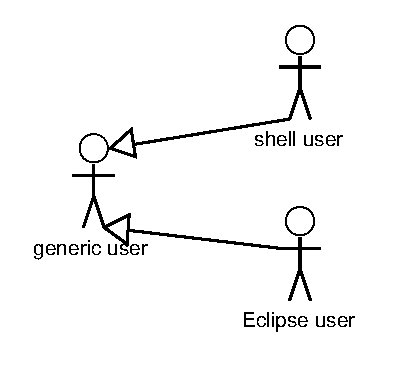
\includegraphics[width=0.3\textwidth]{images/Use_Case_Models/actors}
 \caption{Actors}
 \label{fr_fg:Actors}
\end{figure}
\par
As the software partly integrates with the Eclipse IDE, one type of actor is the \textit{Eclipse user}. He has experience in using Eclipse and has worked with plug-ins before. He wants the plug-in interface to be intuitive and expects a similar behavior he is used to from other plug-ins. He is accustomed to control every software feature out of Eclipse and does not want to have to open external programs.
\par
The \textit{shell user} is the user who controls the software using the system shell. He has used Windows or Linux shells before as well as other command line programs and is used to their respective characteristics. He wants a well-written reference manual and on line help with subcommand and option listing.
\par
In the following use case models often a \textit{generic user} is used, because Eclipse and shell users participate in the same use cases. In these cases, both are generalized to the \textit{generic user}.

\subsection{Use case description} \label{fr:Use case description}
\subsubsection{Preface}
In the rest of this section the functional \gl[specification]{specification} is described. To clarify the functional requirements, a use case analysis is used. There is no common understanding of the purpose of use cases. On the one hand, they are used to show the key functions of the specified software -- the key functions a customer wants to be implemented. On the other hand, they are used to describe the sequence of actions clearly. For the following use case description both aspects are needed.
\par
For the description of the key functions, key use cases are applied. They summarize smaller use cases and allow an overview. These use cases are defined in section~\ref{fr:Key use cases}. Besides the key use cases, standard use cases are employed to describe the functions in detail.

\subsubsection{Predefinitions}
\paragraph{Use case descriptions}
Each standard use case comes with a use case description. The use case description consists of the following items:
\begin{itemize}
  \item Actor
  \item Preconditions
  \item Regular sequence
  \item Other sequences
  \item Postconditions
  \item Possible exceptions
\end{itemize}
\par
The \textit{actor} is the person performing the use case. The actors are described in section~\ref{fr:Actors}.
\par
The \textit{preconditions} describe the circumstances needed to start the use case. This can be a state of the software, an open dialog box or the successful termination of another use case.
\par
The \textit{regular sequence} is the description of the normal steps of the use case. It states how the actor interacts with the software, which input is made and which feedback is returned by the software. It is assumed that the sequence is successfully finished without errors. 
%If there are other possible paths, they are described in \textit{other sequences}.
\par
If there are short cuts or small modifications possible for the regular sequence, they are described in \textit{other sequences} too. Also the cancellation of a use case belongs to this section.
\par
The \textit{postconditions} describe the state of the software and -- if affected -- data after the regular sequence is successfully finished. If there are other possible sequences, the \textit{postconditions} describe the state of the software after each of these sequences.
\par
The \textit{possible exceptions} are used to specify sequences where errors occur. They can be caused by mistakes of the actor, file system errors or other states which cause the sequences to be aborted.
\par
Beginning with the section~\ref{fr:General preconditions} general assumptions are described that hold true for every use case. An explicit \gl[statement]{statement} in the use case description can override these assumptions for a particular use case.

\paragraph{General preconditions} \label{fr:General preconditions}
Considering the Eclipse user, Eclipse must be started. The plug-in must be installed correctly and must not be disabled. A Eclipse \gl[project]{project} must be opened.

\paragraph{General other sequences}
For the use cases of the Eclipse user it is assumed, that every use case which includes interaction with a dialog, can be stopped immediately by clicking the Cancel button in the dialog.
\par
There are often several ways to open a dialog or to execute a command in Eclipse. In most cases only one way is described for simplicity. Some are listed here, because they are explicitly used:
\begin{itemize}
  \item the Eclipse dialog \eclui{Properties} can be opened using the context menu of the dialog or the menu \eclui{Project}
  \item the context menu of a \gl[code file]{code file} can be opened in the \eclui{Package Explorer} and in the \eclui{Navigator}
  \item the context menu can be opened using a right click or the Context Menu Key on the keyboard
\end{itemize}

\paragraph{General postconditions}
If it is stated that something -- e.g. a \gl[test session]{test session} -- is \textit{saved} the changes are stored persistently in the related \gl{session container}.

\paragraph{General possible exceptions}
The general behavior of the software in abnormal situations is described in the section~\ref{nf:Robustness and failure behavior}.
\par
If a session container could not be updated or created -- e.g. due to lack of access permissions or low disk space -- an error message is shown to inform the actor.

\clearpage
\subsubsection{Key use cases} \label{fr:Key use cases}
\begin{figure}[htp]
 \centering
 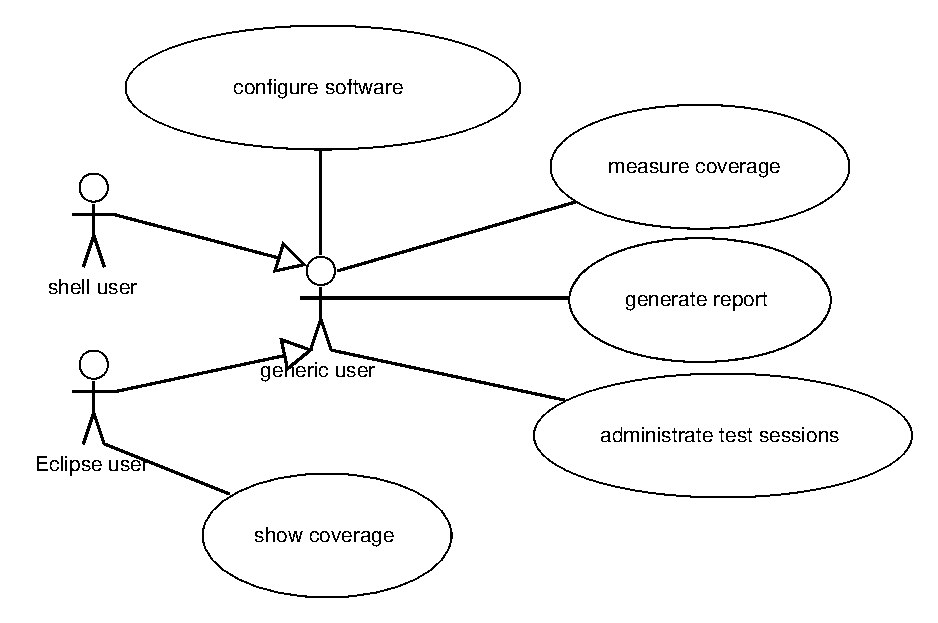
\includegraphics[width=0.7\textwidth]{images/Use_Case_Models/keyusecases}
 \caption{Key use cases}
 \label{fr_fg:Key use cases}
\end{figure}
This diagram shows the key use cases of the software. As introduced in section~\ref{fr:Actors}, there is an Eclipse user and a shell user. Both are specialized from the generic user.
\par
The key use cases summarize a block of functionality and can be subdivided into smaller standard use cases. These are:
\begin{itemize}
  \item Measure coverage (see section~\ref{fr:Measure coverage})
  \item Show coverage (see section~\ref{fr:Show coverage})
  \item Administrate test sessions (see section~\ref{fr:Administrate test sessions})
  \item Generate report (see section~\ref{fr:Use case: generate report})
  \item Configure software (see section~\ref{fr:Configuration})
\end{itemize}

\clearpage
\subsubsection{Measure coverage} \label{fr:Measure coverage}
\begin{figure}[htp]
 \centering
 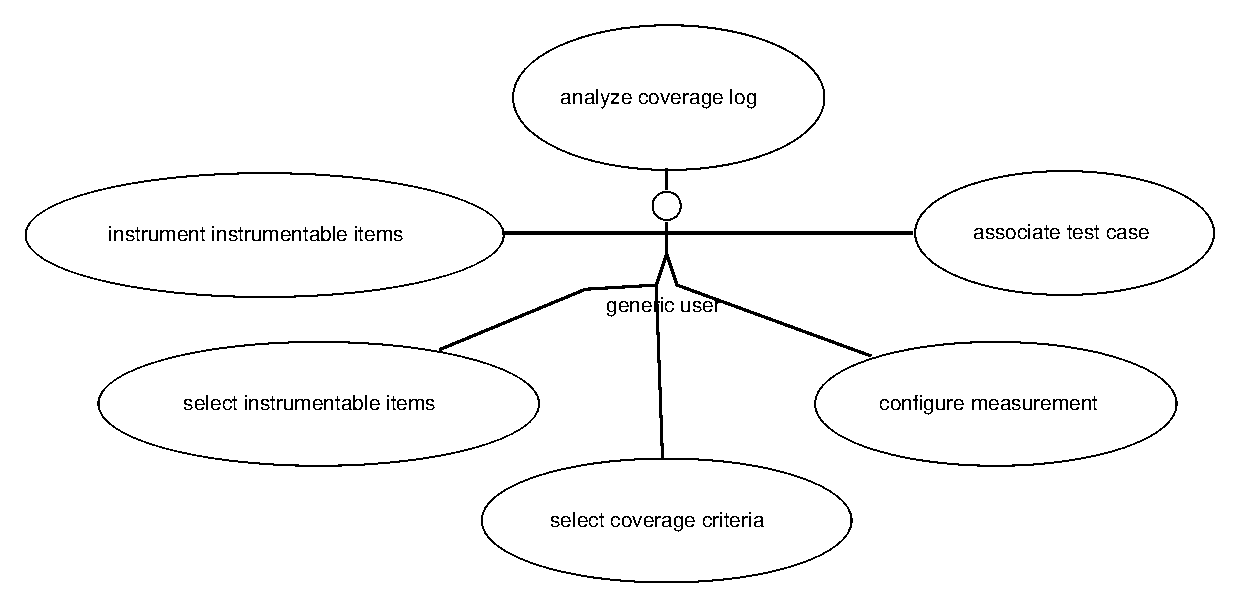
\includegraphics[width=0.8\textwidth]{images/Use_Case_Models/measurecoverage}
 \newline
 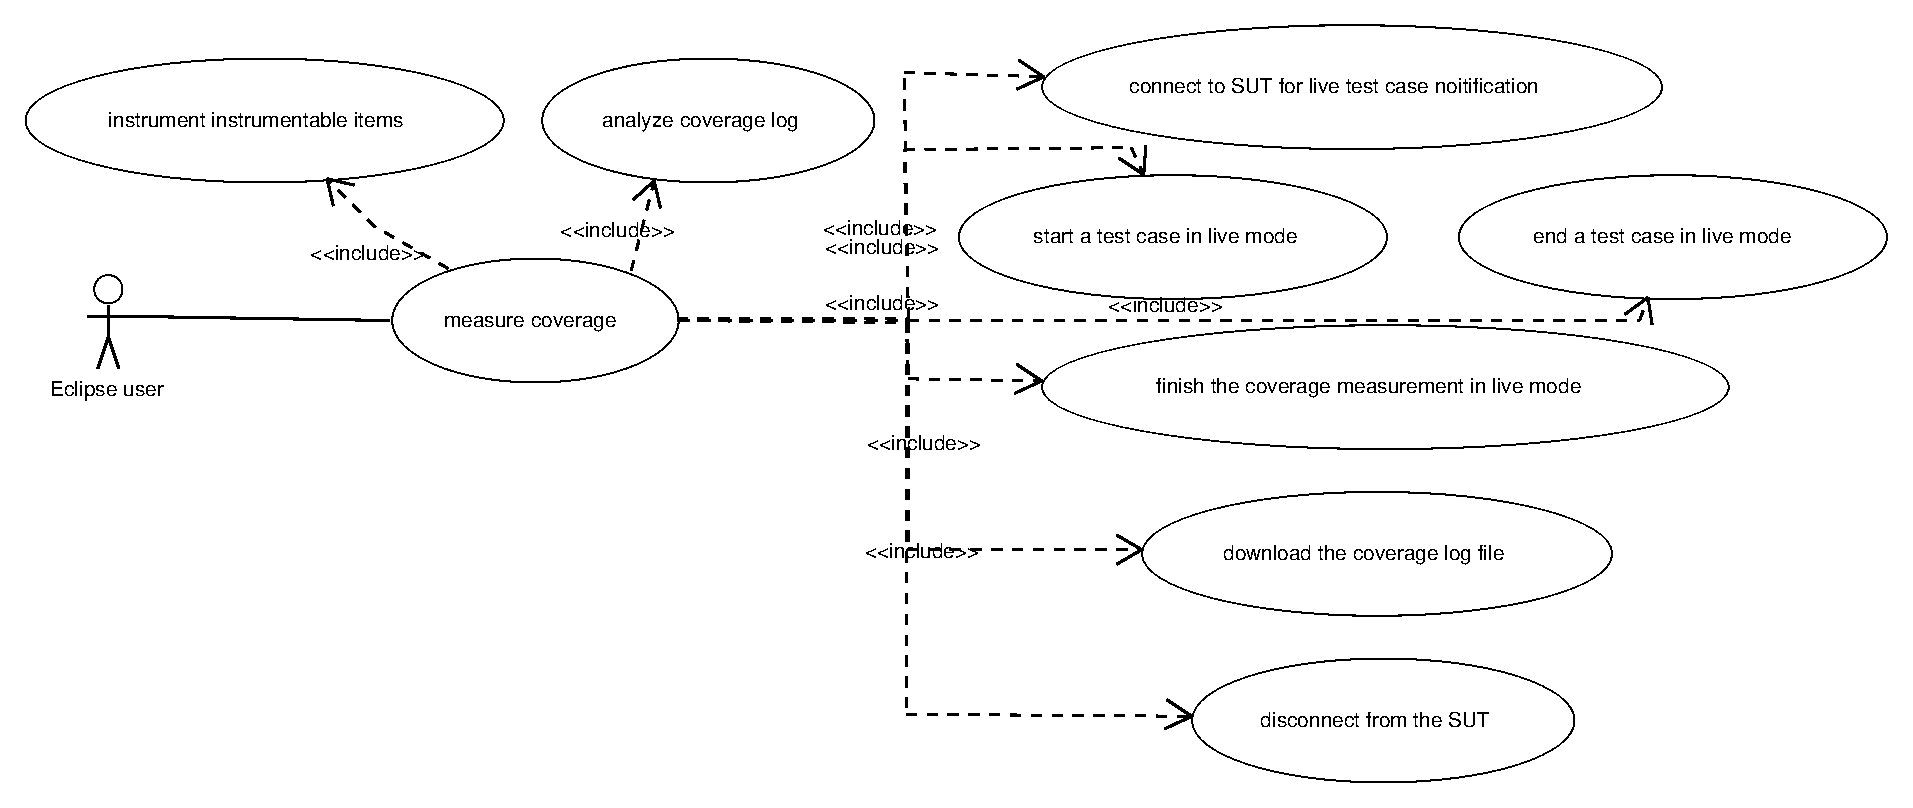
\includegraphics[width=1.0\textwidth]{images/Use_Case_Models/measurecoverageEclipse}
 \caption{Use cases related to measuring coverage}
 \label{fr_fg:Use cases related to measuring coverage}
\end{figure}

\paragraph{Use case: select instrumentable items} \label{fr:Use case: select instrumentable items}
\subparagraph{Actor}
The actor of this use case is the Eclipse user (see section~\ref{fr:Actors}).
\subparagraph{Preconditions}
The actor has opened an Eclipse project containing at least one \gl[instrumentable item]{instrumentable item}.
\subparagraph{Regular sequence}
The actor selects one or more instrumentable items -- e.g. in the \eclui{Package Explorer} -- and clicks on the check box menu item \eclui{Use For Coverage Measurement} in the context menu.
\par
To deselect instrumentable items, the actor repeats the described procedure and clicks on the context menu item \eclui{Use For Coverage Measurement} again.
\subparagraph{Other sequences}
There are no other sequences possible for this use case.
\subparagraph{Postconditions}
Selecting or deselecting an instrumentable item has an recursive effect on all its sub items: for example, selecting a package causes all its sub packages and types to be selected, too. The same applies for the deselecting. If an instrumentable item had been selected before and a parent item is selected later, the originally selected item remains selected.
\par
In the \eclui{Package Explorer}, the icons of the selected instrumentable items change to \eclui{Used For Coverage Measurement} state.
\par
If the actor has deselected instrumentable items, the icon changes to the normal state. (see section~\ref{ui:Package and file states})
\subparagraph{Possible exceptions}
There are no special possible exceptions to be considered for this use case.

\paragraph{Use case: select coverage criteria}
\subparagraph{Actor}
The actor of this use case is the Eclipse user (see section~\ref{fr:Actors}).
\subparagraph{Preconditions}
If the actor has not changed the coverage criteria of a project, all coverage criteria are selected.
\subparagraph{Regular sequence}
The actor opens the \eclui{Project Properties} dialog for the particular project. Then he clicks on the item \eclui{\gbt}. Here the actor can select which coverage criteria he wants to measure. To add a criterion for measurement, he activates the related check box. Deactivating a check box means that the corresponding \gl[coverage criterion]{coverage criterion} will not be measured. It is not possible to deselect all check boxes and apply the changes.
\par
After the actor has made his choice, he clicks on the button \eclui{OK}. The dialog \eclui{Properties} closes.
\subparagraph{Other sequences}
There are no other sequences possible for this use case.
\subparagraph{Postconditions}
At least one coverage criterion is selected for the edited Eclipse project. The software saves this selection. In addition to that, the software checks whether the already instrumented \gl[instrumentable item]{instrumentable items} must be reinstrumented for the new selection of coverage criteria.
\subparagraph{Possible exceptions}
If the actor has deselected all check boxes the dialog prohibits the click on \eclui{OK}.

\paragraph{Use case: instrument instrumentable items} \label{fr:Use case: instrument instrumentable items}
\subparagraph{Actor}
The actor of this use case is the Eclipse user (see section~\ref{fr:Actors}).
\subparagraph{Preconditions}
There are no special preconditions needed for this use case.
\subparagraph{Regular sequence}
The actor uses the menu \eclui{Project} and the menu item \eclui{Instrument Project\dots} to explicitly instrument the selected instrumentable items. A dialog opens and asks the actor to enter the target path for instrumented \gl[code file]{code files}. The actor puts in a valid path he has write access to. With a click on the button \eclui{Instrument} he starts the \gl[instrumentation]{instrumentation} process.
\par
While this process is running, a progress bar appears to inform the actor about the progress of the instrumentation process. The Eclipse integrated progress bar is used for this purpose.
\subparagraph{Other sequences}
This use case is implicitly started by the use case \textit{measure coverage} (see section~\ref{fr:Use case: measure coverage}). In this case, the default target folder of the project for instrumented code files is used and the dialog is not displayed (see section~\ref{fr:Instrumentation process}).
\par
If there are no instrumentable items selected for coverage measurement, the software opens a dialog box to ask the actor, whether he wants to instrument every instrumentable item or wants to cancel.
\subparagraph{Postconditions}
If the use case is explicitly started by the user, a new \gl{code base} is created having the date and time of the end of the instrumentation process. A \gl{MAST} is created of the source files. A new \gl{session container} is created, containing the code base and the MAST. The session container is stored. In the \eclui{Test Sessions} view the new code base is selected. It has got no test session. All code files which are \eclui{Used For Coverage Measurement} are instrumented and stored at the given target path. All other source files are just copied.
\par
The same procedure is used, if this use case is implicitly started by the use case \textit{measure coverage}. The only exception is made, if no changes were made at the source files of the project since the last start of \textit{measure coverage} for this project and the selection of the code files \eclui{Used For Coverage Measurement} has not changed. In this case, the last selected code base can be used again.
\subparagraph{Possible exceptions}
If the instrumented code files could not be written -- e.g. due to lack of access permissions or low disk space -- an error message is shown to inform the actor.

\paragraph{Use case: measure coverage} \label{fr:Use case: measure coverage}
\subparagraph{Actor}
The actor of this use case is the Eclipse user (see section~\ref{fr:Actors}).
\subparagraph{Preconditions}
At least one coverage criterion is activated for measurement. There is an \gl[entry point]{entry point} in the current project.
\subparagraph{Regular sequence}
The actor navigates to the entry point for which he wants to start the coverage measurement. He clicks on the \eclui{Coverage Button} (see figure~\ref{ui_fg:Coverage button}) and at the appearing menu on the button \eclui{Coverage As\dots{}}, \eclui{Java-Application}.
\par
If no code file of this project has been changed since the last start of this use case for the same project and the selection of the code files \eclui{Used For Coverage Measurement} has not changed, no instrumentation is needed. Otherwise, the software will implicitly start the use case \textit{instrument instrumentable items} (see section~\ref{fr:Use case: instrument instrumentable items}) and a new code base will be created.
\par
After having instrumented all the required files, the software rebuilds the instrumented \gl[code file]{code files} and starts the \gl[SUT]{SUT} using the selected entry point.
\par
After the instrumented project has terminated, the software proceeds with the measurement calculation of the covered elements.
\subparagraph{Other sequences}
If the actor has not selected any instrumentable item for coverage measurement, the software opens a dialog box to ask the actor, whether he wants to instrument every instrumentable item or wants to cancel.
\par
If the entry point has been used for coverage measurement before, the list of the \eclui{Coverage Button} contains this entry so that the actor can use this entry directly instead of using the buttons \eclui{Coverage As\dots{}}, \eclui{Java-Application} again.
\par
Additionally, the \eclui{Coverage} dialog (see section~\ref{ui:Launching}) contains entries for coverage measurements used in past. The actor can use this dialog to start a coverage measurement too. He selects the entry in the entry list on the left and clicks on the button \eclui{Coverage}.
\subparagraph{Postconditions}
The result of the coverage measurement run is a \gl[coverage log]{coverage log}. The use case \textit{analyze coverage log} (see section~\ref{fr:Use case: analyze coverage log}) is implicitly started for this coverage log. This use case produces a test session for the measurement.
\par
The software has saved the results of the coverage measurement in a new test session. This test session has the name \textit{New test session} and a number as suffix if needed for uniqueness. The \eclui{Test Sessions} view (see figure~\ref{ui_fg:Session view}) contains the new test session which is automatically selected. All test cases of the new test session are shown in the list of test cases. They are all automatically activated.
\par
If there had not been at least one instrumentable item selected for coverage measurement and the software had selected all after request, then the state of them changes to \eclui{Used for Coverage Measurement} and the \eclui{Package Explorer} updates their icons.
\subparagraph{Possible exceptions}
If there are errors in the process, the process will be canceled and an error message will be shown. Possible errors might be:
\begin{itemize}
  \item I/O errors while instrumenting
  \item compile errors
  \item errors starting the entry point
  \item access permissions or low disk space when writing the \gl{coverage log}
\end{itemize}

\paragraph{Use case: associate test case}
\subparagraph{Purpose}
The actor wants the software to start a named test case, when the control flow passes a specific line in a code file, e.g. the actor has written a test script which calls several methods of several test classes. Test cases should be defined for each of these method calls.
\subparagraph{Actor}
The actor of this use case is the Eclipse user (see section~\ref{fr:Actors}).
\subparagraph{Preconditions}
There is a code file in an open Eclipse project which contains the code the actor wants to add test case notifications to.
\subparagraph{Regular sequence}
The actor navigates to the code file and positions the cursor before the line of the code file where the test case should start. Then he uses the menu items \eclui{Source}, \eclui{\gbt Test Case Notification}, \eclui{Start Test Case With Name And Comment} (see section~\ref{ui:Test case notification}). The software adds an import declaration in the file and adds a new code line at the position of the cursor:
\begin{quote}
  \code{Protocol.startTestCase("\%NAME\%", "\%COMMENT\%");}
\end{quote}
\par
The actor changes \code{"\%NAME\%"} and \code{"\%COMMENT\%"} to the name and the comment of the test case. The software is ordered to start a new test case when this method is called in the coverage measurement.
\par
To define the end of a test case, the actor uses the menu items \eclui{Source}, \eclui{\gbt Test Case Notification}, \eclui{End Test Case With Name} (see section~\ref{ui:Test case notification}). The software adds a new code line:
\begin{quote}
  \code{Protocol.endTestCase("\%NAME\%");}
\end{quote}
\par
The actor changes the \code{"\%NAME\%"} to the name of the test case started before and saves the file.
\subparagraph{Other sequences}
If the actor wants multiple test cases, he uses this procedure at different lines of the code file. He can also associate test cases in other code files.
\par
If the actor only wants to have one test case for the whole test script, he must not add a special statement anywhere. The software then treats the whole measurement as one test case. (see section~\ref{fr:Test sessions and test cases})
\par
There are also other test case notification forms possible that have the same effect. These are described in section~\ref{fr:Test sessions and test cases}. The start of a test case implies the end of the prior test case.
\par
If the actor is more advanced, he can write the statement into the source code on his own. In this case he must add the JAR containing the \code{Protocol} class to the class path of the related Eclipse project too.
\subparagraph{Post conditions}
The software or the actor has added the JAR containing the \code{Protocol} class to the class path of the Eclipse project. The code file is prepared for measurement with test case association.
\subparagraph{Possible exceptions}
There are no special possible exceptions to be considered for this use case.

\paragraph{Use case: analyze coverage log} \label{fr:Use case: analyze coverage log}
\subparagraph{Actor}
The actor of this use case is the Eclipse user (see section~\ref{fr:Actors}).
\subparagraph{Preconditions}
The actor has used the use case \textit{instrument instrumentable items} and has run the compiled SUT on his own and without Eclipse support. In the consequence there is a coverage log related to an Eclipse project.
\par
If the actor has instrumented the code files out of Eclipse, the actor has to import the \gl{session container} with the corresponding \gl{code base} first (see section~\ref{fr:Use case: import session container}).
\par
Anyway, there is a code base loaded in Eclipse and the source files of this code base were compiled and executed. A \gl{coverage log} file was created.
\subparagraph{Regular sequence}
The actor activates the \eclui{Test Sessions} view (see figure~\ref{ui_fg:Session view}). In the view, he clicks on the button \eclui{Import Coverage Log}. The import dialog for session containers opens.
\par
In the dialog the actor specifies the coverage log. Moreover he must state a name and can type a comment for the test session that will be created. After that, he clicks on \eclui{Finish}. The dialog closes. (see figure~\ref{ui_fg:Import coverage log})
\subparagraph{Other sequences}
The dialog for importing a \gl{coverage log} file can also be opened by using the default Eclipse import dialog. For example this can be opened using the menu \eclui{File} and the item \eclui{Import\dots{}}. There the actor selects the item \eclui{\gbt Coverage Log} in the group \eclui{Other} and clicks on \eclui{Next}.
\subparagraph{Post conditions}
The software processes the given coverage log and creates a new test session with the given name and comment. The test session is assigned to the corresponding code base. The test session is saved in the \gl{session container}.
\par
In the new test session is selected in the \eclui{Test Sessions} view (see figure~\ref{ui_fg:Session view}). All its test cases are shown in the list of the test cases and are selected.
\subparagraph{Possible exceptions}
If there is no \gl{code base} in Eclipse, the new coverage log belongs to, an error message is shown.
\par
If the test session is not related to the Eclipse project of the code base, the code highlighting won't be possible (see section~\ref{fr:Use case: show covered code}) but the coverage results can be examined (see section~\ref{fr:Use case: show coverage measurement}).
\par
If there are errors processing the coverage log, the process is interrupted and an error message is shown.

\paragraph{Use case: configure measurement}
The following use cases contains the configuration of the measurement behavior. It is described in section~\ref{fr:Configuration}.

\paragraph{Use case: connect to an SUT for live test case notification} \label{fr:Use case: connect to an SUT for live test case notification}

\subparagraph{Actor} The actor of this use case is the Eclipse user
(see section~\ref{fr:Actors}).

\subparagraph{Preconditions} The instrumented SUT has been configured
to support the live test case notification and is running. The
\eclui{Test Case Notification} view is open.

\subparagraph{Regular sequence} The actor enters the host name and
port to connect to and clicks the \eclui{Connect} button.

\subparagraph{Other sequences}
There are no other sequences possible for this use case.

\subparagraph{Postconditions}
The view is connected to the running SUT.

\subparagraph{Possible exceptions} If there was a network error, an
error message is shown. 

If the CodeCover MBean is not available on the server, the client
waits until a CodeCover MBean is registered; all operations except
disconnecting will stay disable until a CodeCover MBean is registered
on the Server.

\paragraph{Use case: start a new test case in live mode} \label{fr:Use case: start a new test case in live mode}

\subparagraph{Actor} The actor of this use case is the Eclipse user
(see section~\ref{fr:Actors}).

\subparagraph{Preconditions} A connection to a running SUT is
established (see use case \ref{fr:Use case: connect to an SUT for live
  test case notification}). The \eclui{Test Case Notification} view is
open. The coverage measurement in the current SUT run is not finished.

\subparagraph{Regular sequence} The actor enters a test case name in
the text field of the view and clicks the \eclui{Start} button.

\subparagraph{Other sequences}
There are no other sequences possible for this use case.

\subparagraph{Postconditions}
The test case has been started.

\subparagraph{Possible exceptions}
If there was a network error, an error message is shown.

\paragraph{Use case: end the current test case in live mode} \label{fr:Use case: end the current test case in live mode}

\subparagraph{Actor} The actor of this use case is the Eclipse user
(see section~\ref{fr:Actors}).

\subparagraph{Preconditions} A connection to a running SUT is
established (see use case \ref{fr:Use case: connect to an SUT for live
  test case notification}). The \eclui{Test Case Notification} view is
open. A test case is started.

\subparagraph{Regular sequence} The actor clicks the \eclui{End}
button in the \eclui{Test Case Notification} view.

\subparagraph{Other sequences}
There are no other sequences possible for this use case.

\subparagraph{Postconditions}
The test case has been ended.

\subparagraph{Possible exceptions}
If there was a network error, an error message is shown.

\paragraph{Use case: finish coverage measurement in live mode} \label{fr:Use case: finish coverage measurement in live mode}

\subparagraph{Actor} The actor of this use case is the Eclipse user
(see section~\ref{fr:Actors}).

\subparagraph{Preconditions} A connection to a running SUT is
established (see use case \ref{fr:Use case: connect to an SUT for live
  test case notification}). The \eclui{Test Case Notification} view is
open.

\subparagraph{Regular sequence} The actor clicks the \eclui{Finished}
button in the \eclui{Test Case Notification} view.

\subparagraph{Other sequences}
There are no other sequences possible for this use case.

\subparagraph{Postconditions}
The measurement has been finished.

\subparagraph{Possible exceptions}
If there was a network error, an error message is shown.

\paragraph{Use case: download the coverage log file} \label{fr:Use case: download the coverage log file}

\subparagraph{Actor} The actor of this use case is the Eclipse user
(see section~\ref{fr:Actors}).

\subparagraph{Preconditions} A connection to a running SUT is
established (see use case \ref{fr:Use case: connect to an SUT for live
  test case notification}). The \eclui{Test Case Notification} view is
open. The coverage measurement has been finished.

\subparagraph{Regular sequence} The actor clicks the \eclui{Download}
button in the \eclui{Test Case Notification} view.

\subparagraph{Other sequences}
There are no other sequences possible for this use case.

\subparagraph{Postconditions} The coverage log file is downloaded and has the same
base name as the file written on the system running the SUT and the
same location as if the execution was local and triggered by \gbt\
Eclipse plug-in.

\subparagraph{Possible exceptions} If there was a network or file
access error, an error message is shown.

\paragraph{Use case: disconnect from the SUT in live mode} \label{fr:Use case: disconnect from the SUT in live mode}

\subparagraph{Actor} The actor of this use case is the Eclipse user
(see section~\ref{fr:Actors}).

\subparagraph{Preconditions} A connection to a running SUT is
established (see use case \ref{fr:Use case: connect to an SUT for live
  test case notification}). The \eclui{Test Case Notification} view is
open.

\subparagraph{Regular sequence} The actor clicks the \eclui{Disconnect}
button in the \eclui{Test Case Notification} view.

\subparagraph{Other sequences}
There are no other sequences possible for this use case.

\subparagraph{Postconditions} The connection to the SUT is closed.

\subparagraph{Possible exceptions} If there was a network error, a
warning is shown.


\clearpage
\subsubsection{Show coverage} \label{fr:Show coverage}
\begin{figure}[htp]
 \centering
 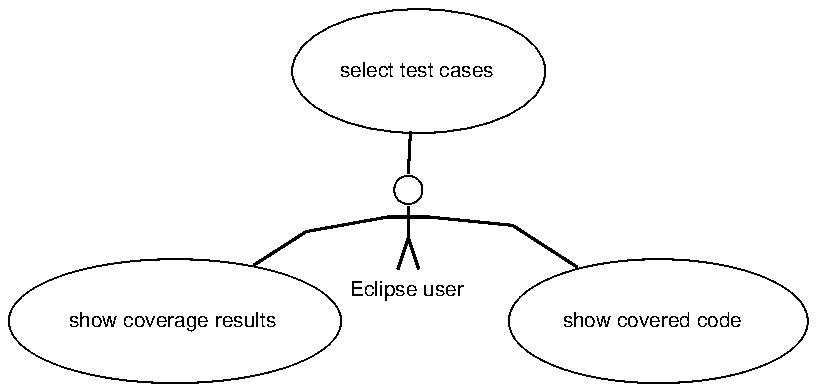
\includegraphics[width=0.6\textwidth]{images/Use_Case_Models/showcoverage}
 \caption{Use cases related to showing coverage}
 \label{fr_fg:Use cases related to showing coverage}
\end{figure}

\paragraph{Use case: select test cases} \label{fr:Use case: select test cases}
\subparagraph{Actor}
The actor of this use case is the Eclipse user (see section~\ref{fr:Actors}).
\subparagraph{Preconditions}
There is at least one test session in Eclipse which has at least one test case. 
\subparagraph{Regular sequence}
The actor opens the \eclui{Test Sessions} view (see figure~\ref{ui_fg:Session view}). Then he selects the related \eclui{Code base}.
\par
Now the actor can activates all test cases he wants to view the coverage results of, using the \eclui{Activated} check boxes. The rest of the test cases' check boxes have to be deactivated.
\subparagraph{Other sequences}
The actor can select test cases of different test sessions. To select all test cases of a test session, the actor uses the \eclui{Activated} check box of the specific test session.
\par
There are some other sequences possible to activate test cases -- e.g. using the context menu in the \eclui{Test Sessions} view (see section~\ref{ui:Test sessions view}).
\subparagraph{Postconditions}
The source code highlighting and the coverage view are refreshed if needed, based on the results of the selected test cases.
\subparagraph{Possible exceptions}
There are no special possible exceptions to be considered for this use case.

\paragraph{Use case: show coverage measurement} \label{fr:Use case: show coverage measurement}
\subparagraph{Actor}
The actor of this use case is the Eclipse user (see section~\ref{fr:Actors}).
\subparagraph{Preconditions}
The actor has selected test cases of test sessions belonging to the same code base (see use case \textit{select test cases}, section~\ref{fr:Use case: select test cases}).
\subparagraph{Regular sequence}
The actor activates the \eclui{Coverage} view of the plug-in (see figure~\ref{ui_fg:Coverage view}). At this view he has an overview of all instrumented instrumentable items in a hierarchical order. He can expand an item of the hierarchy to examine the coverage results of its sub items.
\par
The result columns show the measured results of the coverage by criterion. Only the criteria that are measured are shown in this view.
\par
To order the lines of the tree table ascending or descending, the actor clicks respectively clicks twice on the specific column header. The lines of items are then sorted within their parent item in the tree table.
\subparagraph{Other sequences}
There are no other sequences possible for this use case.
\subparagraph{Postconditions}
There are no possible post conditions of this use case.
\subparagraph{Possible exceptions}
There are no special possible exceptions to be considered for this use case.

\paragraph{Use case: show covered code} \label{fr:Use case: show covered code}
\subparagraph{Actor}
The actor of this use case is the Eclipse user (see section~\ref{fr:Actors}).
\subparagraph{Preconditions}
The actor has selected test cases of test sessions belonging to the same code base (see use case \textit{select test cases}, section~\ref{fr:Use case: select test cases}). The code base of the test sessions selected is still the current one, which means, no code file has been changed since the instrumentation of the code files.
\subparagraph{Regular sequence}
The actor navigates to the code file in which the coverage results are to be displayed by source code highlighting. Then he opens the code file in an editor.
\subparagraph{Other sequences}
There are no other sequences possible for this use case.
\subparagraph{Postconditions}
The software highlights the elements of the code according to results of the measurement of the selected coverage criteria. The highlighting rules are specified in section~\ref{ui:Source code highlighting} in detail.
\subparagraph{Possible exceptions}
If a code file has changed since the coverage run of the test session, the highlighting can not be shown. Therefore the software has to check, if the code file has the same content as the code file used for the related coverage run.
\par
If the actor changes a code file, the highlighting is not possible anymore. If he revokes his changes, the software shows the highlighting again.

\clearpage
\subsubsection{Administrate test sessions} \label{fr:Administrate test sessions}
\begin{figure}[htp]
 \centering
 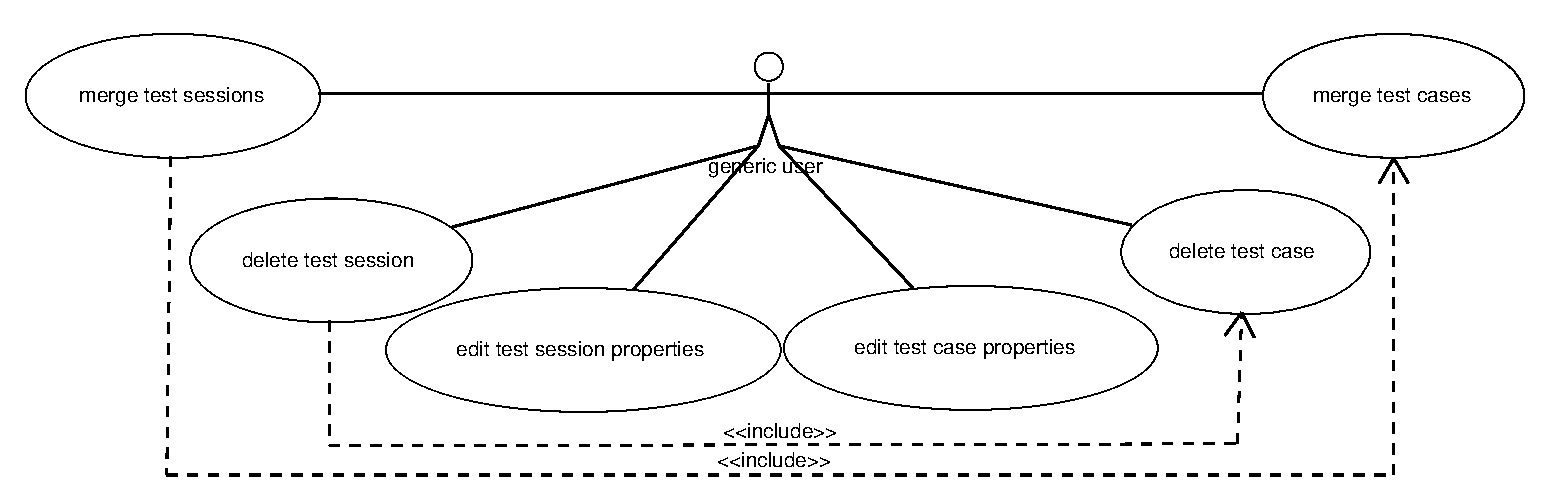
\includegraphics[width=0.95\textwidth]{images/Use_Case_Models/administratetestsessions} \newline
 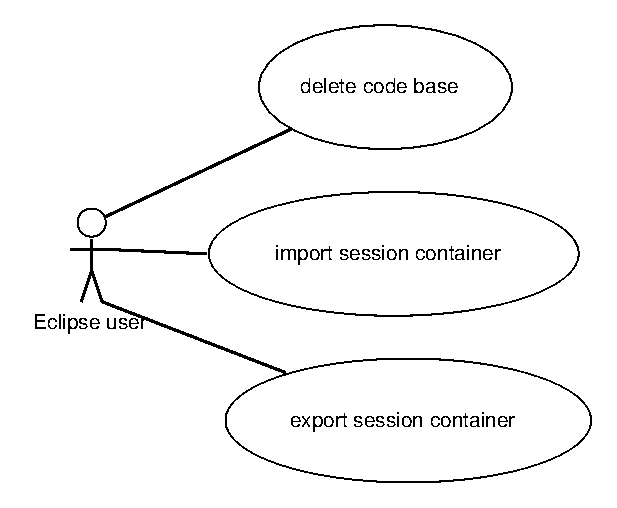
\includegraphics[width=0.4\textwidth]{images/Use_Case_Models/Eclipseadministration}
 \caption{Use cases related to administrating test sessions}
 \label{fr_fg:Use cases related to administrating test sessions}
\end{figure}

\paragraph{Preface}
These use cases are based on other use cases described before. By measuring the coverage, the software creates a test session containing associated test cases. They are the basis of analysis and can be edited in several ways. The test sessions and test cases can be merged and their properties can be altered. Test cases can be deleted from a test session and whole test sessions with all included test cases can be deleted.
\par
To use the Eclipse plug-in and the batch interface side by side, import and export functionality is supported by the Eclipse plug-in. General definitions regarding \gl[test session]{test sessions} and test cases are made in the section~\ref{fr:Test sessions and test cases}.

\paragraph{Use case: import session container} \label{fr:Use case: import session container}
\subparagraph{Actor}
The actor of this use case is the Eclipse user (see section~\ref{fr:Actors}).
\subparagraph{Preconditions}
There must be at least one \gl[session container]{session container} in the file system. This can be either created by a coverage measurement in Eclipse or using the batch mode (see section~\ref{fr:Batch interface}).
\subparagraph{Regular sequence}
The actor activates the \eclui{Test Sessions} view (see figure~\ref{ui_fg:Session view}). In the view, he clicks on the button \eclui{Import Test Session}. The import dialog for session containers opens (see figure~\ref{ui_fg:Import session container}). In this dialog, the actor specifies the path to the session container and selects the related Eclipse project. Finally the actor clicks on the button \eclui{Finish}. The dialog closes.
\subparagraph{Other sequences}
The dialog for importing a session container can also be opened by using the default Eclipse import dialog. For example this can be opened using the menu \eclui{File} and the item \eclui{Import\dots{}}. There the actor selects the item \eclui{\gbt Session Container} in the group \eclui{Other} and clicks on \eclui{Next}.
\par
If the code base of the session container is not related to an Eclipse project, the actor needn't select a project.
\subparagraph{Postconditions}
The code base of the session container is imported into Eclipse.
\par 
If the session container has got test session(s), they are imported too. In this case, one of the imported test sessions is selected in the \eclui{Test Sessions} view (see figure~\ref{ui_fg:Session view}). All its test cases are shown in the list of the test cases and are activated.
\par
All information needed to use the session container in Eclipse for future are saved.
\subparagraph{Possible exceptions}
If the \gl{code base} of the session container is not related to the specified project, the code highlighting won't be possible (see section~\ref{fr:Use case: show covered code}) but the coverage results can be examined (see section~\ref{fr:Use case: show coverage measurement}).
\par
If there are errors loading the session container, the process is interrupted and an error message is shown.

\paragraph{Use case: export session container}
\subparagraph{Actor}
The actor of this use case is the Eclipse user (see section~\ref{fr:Actors}).
\subparagraph{Preconditions}
There must be at least one test session in Eclipse.
\subparagraph{Regular sequence}
The actor selects the code base and its test sessions he wants to export in the \eclui{Test Sessions} view (see figure~\ref{ui_fg:Session view}) and clicks on the button \eclui{Export} in the tool bar.
\par
The export dialog opens (see figure~\ref{ui_fg:Export Test Session}). The selected code base and the selected test sessions are preselected in the dialog, but the actor can also select more test sessions. He changes the \eclui{Type} to \eclui{\gbt session container}, chooses a destination and clicks on \eclui{Finish}. The dialog closes.
\subparagraph{Other sequences}
The dialog for exporting a test session can also be opened by using the default Eclipse export dialog. This dialog can for example be opened using the menu \eclui{File} and the item \eclui{Export\dots{}}. In the selection dialog the actor selects the item \eclui{\gbt Coverage Result Export} in the group \eclui{Other} and clicks on \eclui{Next}.
\subparagraph{Postconditions}
A session container is created at the specified destination. It contains the code base and all selected test session.
\subparagraph{Possible exceptions}
There are no special possible exceptions to be considered for this use case.

\paragraph{Use case: drop code base}
\subparagraph{Actor}
The actor of this use case is the Eclipse user (see section~\ref{fr:Actors}).
\subparagraph{Preconditions}
There must be at least one code base in Eclipse.
\subparagraph{Regular sequence}
The actor opens the \eclui{Test Sessions} view (see figure~\ref{ui_fg:Session view}), selects the \gl{code base} and clicks on the button \eclui{Drop Code Base}. A dialog opens, requesting the actor if he wants to drop the selected code base out of Eclipse or if he wants to deleted the related \gl{session container} too. The actor clicks on the button \eclui{Drop}. The dialog closes.
\subparagraph{Other sequences}
If the actor wants to drop the code base out of Eclipse and delete the related code base too, he clicks on \eclui{Delete}.
\subparagraph{Postconditions}
The selected code base and all depending test sessions and test cases are removed from the \eclui{Test Sessions} view.
\par
If the actor has chosen \eclui{Delete}, the session container of the code base is deleted in the file system too.
\subparagraph{Possible exceptions}
There are no special possible exceptions to be considered for this use case.

\paragraph{Use case: merge test sessions} \label{fr:Use case: merge test sessions}
\subparagraph{Actor}
The actor of this use case is the Eclipse user (see section~\ref{fr:Actors}).
\subparagraph{Preconditions}
There must be at least two test sessions in Eclipse.
\subparagraph{Regular sequence}
The actor activates the \eclui{Test Sessions} view (see figure~\ref{ui_fg:Session view}). In this view, he selects the  test session, he want to merge and clicks on the button \eclui{Merge}. The dialog \eclui{Test Session Properties} opens (similar to figure~\ref{ui_fg:Test case properties}).
\par
The actor puts in the name and the comment of the merged test session and clicks on the button \eclui{OK}. The dialog closes.
\subparagraph{Other sequences}
There are no other sequences possible for this use case.
\subparagraph{Postconditions}
A new test session with the specified name is created. All test case information from the test sessions selected for merge are copied into the new test session. The new test session is saved.
\par
If some test cases have the same name, they are renamed to \code{test case name (session name 1)}, \code{test case name (session name 2)}.
\par
The new test session appears in the list of the \eclui{Test Sessions} view. The new session and all its test cases are activated.
\subparagraph{Possible exceptions}
If the actor has selected less than two test sessions, the dialog prohibits the click on the button \eclui{Merge}.

\paragraph{Use case: edit test session properties}
\subparagraph{Actor}
The actor of this use case is the Eclipse user (see section~\ref{fr:Actors}).
\subparagraph{Preconditions}
There must be at least one test session in Eclipse.
\subparagraph{Regular sequence}
The actor activates the \eclui{Test Sessions} view (see figure~\ref{ui_fg:Session view}), selects a test session and clicks on the button \eclui{Properties}. The dialog \eclui{Test Session Properties} opens (similar to figure~\ref{ui_fg:Test case properties}).
\par
The actor changes the name and/or the comment of the selected test session. After he has finished editing the properties, he clicks on the button \eclui{OK}. The dialog closes.
\subparagraph{Other sequences}
There are no other sequences possible for this use case.
\subparagraph{Postconditions}
The new name and the new comment of the test session are saved. The name of the test session changes in the list.
\subparagraph{Possible exceptions}
The new name of the test session can not equal to a name of another test session in the session container. The dialog does not allow to save a duplicate name.

\paragraph{Use case: delete test session}
\subparagraph{Actor}
The actor of this use case is the Eclipse user (see section~\ref{fr:Actors}).
\subparagraph{Preconditions}
There must be at least one test session in Eclipse.
\subparagraph{Regular sequence}
The actor opens the \eclui{Test Sessions} view (see figure~\ref{ui_fg:Session view}), selects the related \gl{code base} and the test session. Then he clicks on the button \eclui{Delete}.
\subparagraph{Other sequences}
If the actor wants to drop more than one test session at once, he selects these test cases and clicks on the button \eclui{Delete}. A dialog opens, requesting the actor if he really wants to delete the selected test sessions. The actor clicks on the button \eclui{Delete}. The dialog closes.
\subparagraph{Postconditions}
The selected test sessions are removed from the session container and from the \eclui{Test Sessions} view.
\subparagraph{Possible exceptions}
There are no special possible exceptions to be considered for this use case.

\paragraph{Use case: merge test cases}
\subparagraph{Actor}
The actor of this use case is the Eclipse user (see section~\ref{fr:Actors}).
\subparagraph{Preconditions}
There must be a test session in Eclipse that contains at least two test cases that fit the merging criteria stated in section~\ref{fr:Test sessions and test cases}.
\subparagraph{Regular sequence}
The actor opens the \eclui{Test Sessions} view (see figure~\ref{ui_fg:Session view}), selects the related \gl{code base}, the test session and the test cases. Then he clicks on the button \eclui{Merge}. The dialog \eclui{Test Case Properties} opens (see figure~\ref{ui_fg:Test case properties}).
\par
The actor puts in the name and the comment of the merged test case and clicks on the button \eclui{OK}. The dialog closes.
\subparagraph{Other sequences}
The actor can also use the item \eclui{Merge} in the context menu of the test cases.
\subparagraph{Postconditions}
A new test case with the specified name is created. All information from the selected test cases are copied into the new test case. The test case is saved.
\par
The new test case appears in list of the \eclui{Test Sessions} view.
\subparagraph{Possible exceptions}
If the actor has selected less than two test cases, the button \eclui{Merge Test Cases} is deactivated.

\paragraph{Use case: edit test case properties}
\subparagraph{Actor}
The actor of this use case is the Eclipse user (see section~\ref{fr:Actors}).
\subparagraph{Preconditions}
There must be at least one test case in a test session in Eclipse.
\subparagraph{Regular sequence}
The actor opens the \eclui{Test Sessions} view (see figure~\ref{ui_fg:Session view}), selects the related \gl{code base}, the test session and the test case. Then he clicks on the button \eclui{Properties}. The dialog \eclui{Test Case Properties} opens (see figure~\ref{ui_fg:Test case properties}).
\par
The actor changes the name and/or the comment of the selected test case. After he has finished editing the properties, he clicks on the button \eclui{OK}. The dialog closes.
\subparagraph{Other sequences}
The actor can also use the menu item \eclui{Properties} in the test case's context menu in the \eclui{Test Sessions} view.
\subparagraph{Postconditions}
The new name and the new comment of the test case are saved. The name of the test case is updated in the list.
\subparagraph{Possible exceptions}
If the actor has not selected exactly one test case, the button \eclui{Test Case Properties} is deactivated.
\par The new name of the test case can not equal to a name of another test case in the test session. The dialog does not allow to save a duplicate name.

\paragraph{Use case: delete test case}
\subparagraph{Actor}
The actor of this use case is the Eclipse user (see section~\ref{fr:Actors}).
\subparagraph{Preconditions}
There must be at least one test case in a test session in Eclipse.
\subparagraph{Regular sequence}
The actor opens the \eclui{Test Sessions} view (see figure~\ref{ui_fg:Session view}), selects the related \gl{code base}, the test session and the test case. Then he clicks on the button \eclui{Delete}. A dialog opens, requesting the actor if he really wants to delete the selected test cases. The actor clicks on the button \eclui{Delete}. The dialog closes.
\subparagraph{Other sequences}
The actor can also use the menu item \eclui{Delete} in the test case's context menu in the \eclui{Test Sessions} view.
\subparagraph{Postconditions}
The selected test cases are removed from the list in the \eclui{Test Sessions} view. The test cases are removed from the test session in the session container.
\subparagraph{Possible exceptions}
There are no special possible exceptions to be considered for this use case.

\subsubsection{Use case: generate report} \label{fr:Use case: generate report}
\paragraph{Actor}
The actor of this use case is the Eclipse user (see section~\ref{fr:Actors}).
\paragraph{Preconditions}
There must be at least one test session in Eclipse.
\paragraph{Regular sequence}
The actor selects a \gl{code base} and a set of test sessions in \eclui{Test Sessions} view (see figure~\ref{ui_fg:Session view}). Then he clicks on the button \eclui{Export}. The \eclui{Export} dialog opens (see figure~\ref{ui_fg:Export Test Session}).
\par
The current code base and the selected test sessions are preselected in the dialog, but the actor can also select another code base or other test sessions. He changes the \eclui{Type} to \eclui{Report}, chooses a destination and clicks on \eclui{Next}. The report dialog opens (see figure~\ref{ui_fg:Report dialog}).
\par
The actor clicks on the button \eclui{Finish}. The dialog closes.
\paragraph{Other sequences}
The dialog for generating a report can also be opened by using the default Eclipse export dialog. For example, this can be done using the menu \eclui{File} and the item \eclui{Export\dots{}}. There the actor selects the item \eclui{\gbt Coverage Result Export} in the group \eclui{Other} and clicks on \eclui{Next}.
\paragraph{Post conditions}
A report is generated and stored in the chosen directory. The contents and appearance of the generated report is defined in section~\ref{fr:Report}.
\paragraph{Possible exceptions}
If the report files could not be written -- e.g. due to lack of access permissions or low disk space -- an error message is shown to inform the actor.

\subsection{Batch interface} \label{fr:Batch interface}
\subsubsection{Preface}
To describe the use cases for the actor \textit{shell user}, the shell commands are described. It is recommended that the executable \code{codecover} is contained in the \texttt{PATH} variable of the operating system.
\par
The software can be run in the shell by calling either \code{codecover \%command\% [\%options\%]} or \code{codecover \%option\%}. All available commands are described in the rest of this section. Section~\ref{fr:Batch interface-Command overview} contains an overview about all supported commands.
\par
If the actor wants to use \code{spaces} in arguments -- e.g. file names -- he must take care that the shell he is using parses the file name as one argument. For example he might enclose the file name using quotation marks: \code{"my file name.sql"}.
\par
If the actor has called the software with an unsupported command, the software stops immediately and prints an error message:\\
\code{Command not supported. Use "codecover $--$help" for a command overview.}
\par
If the actor has called the software with a supported command but a wrong option or syntactically wrong parameters, the software stops immediately and prints an error message like this:\\
\code{Wrong argument usage. Use "codecover help \%command\%" for options description.}

\subsubsection{General options}
Using the software without a command some general options are supported. These options can be used by: \code{codecover \%option\%}.
\begin{longtable}{|l|p{11cm}|}\hline
   {\textbf{Option}} &
   {\textbf{Explanation}} \\\hline \hline \endhead
     \verb$--$help|-h & A help page containing this command overview. Has the same effect like \code{codecover help}. \\\hline
     \verb$--$version|-V & Prints out the version of the software. \\\hline
  \caption{General batch options}
  \label{fr_tb:General batch options}
\end{longtable}

\subsubsection{Command overview} \label{fr:Batch interface-Command overview}
For almost every command, either a long or a short version can be used. These commands can be used by \code{codecover \%\textbf{command}\% [\%options\%]}.
\begin{longtable}{|l|p{10cm}|}\hline
   {\textbf{Command}} &
   {\textbf{Description}} \\\hline \hline \endhead
   instrumenter-info|ii & Information of all available instrumenters \\\hline
   instrument|in & \gl[instrumentation]{Instrumentation} of \gl[code file]{code files} \\\hline
   analyze|an & Analysis of a coverage run to create a test session \\\hline
   report|re & Generating a report from a test session \\\hline
   info & Showing the information of a \gl[session container]{session container} and contained test sessions and test cases \\\hline
   merge-sessions|ms & Merging two or more test sessions \\\hline
   alter-session|as & Altering test session information \\\hline
   copy-sessions|cs & Copy test sessions from one session container to another \\\hline
   remove-sessions|rs & Removing test sessions from a session container \\\hline
   merge-test-cases|mc & Merging two or more test cases \\\hline
   alter-test-case|at & Editing test case information \\\hline
   remove-test-cases|rt & Removing test cases from a session container \\\hline
   help|h & A help page containing this command overview or an option and parameter overview a given command. \\\hline
  \caption{Batch command overview}
  \label{fr_tb:Batch command overview}
\end{longtable}

\subsubsection{Global command options}
For every command a set of options is supported. In addition to specific command options, all commands support some global parameterless options. They are not required but change the behavior of the software when used. These commands can be used by \code{codecover \%command\% [\%\textbf{options}\%]}.
\begin{longtable}{|l|p{11cm}|}\hline
   {\textbf{Option}} &
   {\textbf{Explanation}} \\\hline \hline \endhead
     \verb$--$verbose|-v & Orders the software to print more information as usual. For example this can be a description of the actions being done. This option is the opposite of \verb$--$quiet. \\\hline
     \verb$--$quiet|-q & Orders the software not to print information to the shell. This option is the opposite to \verb$--$verbose. \\\hline
     \verb$--$pretend|-p & Orders the software not to perform any actions affecting the data persistently but to print information about what the software would do instead. Using \verb$--$pretend the actor can make sure that his command has the correct syntax and would be successfully executed. \\\hline
     \verb$--$help|-h & Prints an option and parameter overview of the given command. Has the same effect like \code{codecover help \%command\%}. \\\hline
  \caption{General batch options}
  \label{fr_tb:General batch command options}
\end{longtable}

\subsubsection{Instrumenter-info} \label{fr:Batch:Instrumenter-info}
This command allows the actor to get information of the instrumenters, that are available by the software. Using this command, the actor can get to know, which instrumenter fits to his programming language and which additional options are supported.
\par
This command is run by:
\begin{quote}
\code{codecover (instrumenter-info|ii) [options]}
\end{quote}

\begin{longtable}{|l|l|p{73mm}|c|}\hline
   \multicolumn{2}{|l|}{\textbf{Option}} & 
   {\textbf{Parameter and description}} & 
   {\textbf{Default}} \\
   {\textbf{Short}} &
   {\textbf{Long}} &
    & 
   if omitted \\\hline \hline \endhead
   -l & \verb$--$language & the name of the programming language & all \\\hline
  \caption{Options for command instrumenter-info}
  \label{fr_tb:Options for command instrumenter-info}
\end{longtable}

\subsubsection{Instrument} \label{fr:Batch:Instrument}
This command instruments a set of \gl[code file]{code files}. To select the code files, which should be instrumented, a \code{root-directory} must be specified. All code files must be located under this directory. For this reason a \code{default package} would be the best choice.
\par
For a more detailed selection, include patterns can be used. These patterns allow wildcards and are adopted from the \linkwithfootnote{http://ant.apache.org/}{apache ant project}  (see the  \linkwithfootnote{http://ant.apache.org/manual/dirtasks.html}{pattern description}). The actor can specify more than one include pattern, to select the source files for instrumentation. The same way exclude patterns can be specified.
\par
A file will be instrumented, if its relative path matches at least one include pattern, if it has the correct extension for the stated programming language and its relative path matches no exclude pattern.
\par
This command is run by:
\begin{quote}
\code{codecover (instrument|in) [options]}
\end{quote}

\begin{longtable}{|l|l|p{73mm}|c|}\hline
   \multicolumn{2}{|l|}{\textbf{Option}} & 
   {\textbf{Parameter and description}} & 
   {\textbf{Required /}} \\
   {\textbf{Short}} &
   {\textbf{Long}} &
    & 
   {\textbf{Default}} \\\hline \hline \endhead
   -r & \verb$--$root-directory & the root directory of the source files & \x \\\hline
   -l & \verb$--$language & the name of the programming language & \x \\\hline
   -d & \verb$--$destination & the destination directory for the instrumented files& \x \\\hline
   -c & \verb$--$container & the new session container& \x \\\hline
   -I & \verb$--$instrumenter & the unique key of the instrumenter to use & \\\hline
   -a & \verb$--$charset & the character encoding of the source files & system default \\\hline
   -i & \verb$--$include & a relative include pattern; this argument can occur more than one time & all files \\\hline
   -f & \verb$--$includes-file & a file containing a list of relative include patterns separated by new line & \\\hline
   -e & \verb$--$exclude & a relative exclude pattern; this argument can occur more than one time & \\\hline
   -x & \verb$--$excludes-file & a file containing a list of relative exclude patterns separated by new line & \\\hline
   -o & \verb$--$criterion & one of (\code{all}, \code{st}, \code{br}, \code{co}, \code{lo}); this argument can occur more than one time -- once for every criterion & \code{all} \\\hline
   -u & \verb$--$copy-uninstrumented & advices the software to copy all files of the root-directory, that were not instrumented, to the destination & disabled \\\hline
   -D & \verb$--$directive & arguments of the style \code{key=value} to enable special features of the instrumenter; the instrumenter-info command should print out a list of directives, an instrumenter supports & \\\hline
  \caption{Options for command instrument}
  \label{fr_tb:Options for command instrument}
\end{longtable}
\par
The arguments of option \code{criteria} stand for:
\begin{longtable}{|c|l|}\hline
   {\textbf{Criteria abbreviation}} &
   {\textbf{Explanation}} \\\hline \hline \endhead
     \code{all} & all criteria \\\hline
     \code{st} & \gl[statement coverage]{statement coverage} \\\hline
     \code{br} & \gl[branch coverage]{branch coverage} \\\hline
     \code{co} & \gl[condition coverage]{condition coverage} \\\hline
     \code{lo} & \gl[loop coverage]{loop coverage} \\\hline
  \caption{Explanation of the criteria abbreviations}
  \label{fr_tb:Explanation of the criteria abbreviations}
\end{longtable}
\par An example call of the command \code{instrument} is:
\begin{verbatim}
codecover instrument --root-directory "C:\my files\project 1\" --include
"de\foo\pak1\**" --include "de\foo\pak2\dot*.java" --exclude "**\*Test.java"
-d "C:\my files\instrumented\" --language java --criterion st --criterion br
--copy-uninstrumented --container session-container-file.xml
\end{verbatim}
\par
The option \verb$--$\code{copy-uninstrumented} can be used to get a replica of a source directory including resource files like images or configuration files.
\par
If there is more than one instrumenter available for the specified programming language, the software aborts this instrumentation attempt. An error message is printed out like
\begin{quote}
There is more than one instrumenter available for \%programming language\%. Please use the command \code{codecover instrumenter-info} to get to know the unique key of the instrumenter you prefer. Than use the option \code{instrumenter} for this command to exactly specify the instrumenter by its unique key.
\end{quote}
\par
Along with the instrumented code files, the instrumentation process produces a \gl{session container} containing the \gl{code base} and the \gl{MAST}. The new \gl{code base} is has the date and time of the end of the instrumentation process. The code base is stored.

\subsubsection{Analyze} \label{fr:Batch:Analyze}
This command is run by:
\begin{quote}
\code{codecover (analyze|an) [options]}
\end{quote}
\par
This command needs the session container produced by the instrumentation process and the \gl[coverage log]{coverage log} produced by the executed instrumented and compiled program.

\begin{longtable}{|l|l|p{73mm}|c|}\hline
   \multicolumn{2}{|l|}{\textbf{Option}} & 
   {\textbf{Parameter and description}} & 
   {\textbf{Required /}} \\
   {\textbf{Short}} &
   {\textbf{Long}} &
    & 
   {\textbf{Default}} \\\hline \hline \endhead
   -c & \verb$--$container & the session container the coverage data should be added to& \x \\\hline
   -g & \verb$--$coverage-log & the coverage log produced by the executed program &\x  \\\hline
   -n & \verb$--$name & the name of the new test session containing the coverage results & \x \\\hline
   -m & \verb$--$comment & a comment describing the test session & empty \\\hline
   -a & \verb$--$charset & the character encoding of the coverage log file & system default \\\hline
  \caption{Options for command analyze} 
  \label{fr_tb:Options for command analyze}
\end{longtable}
\par
If the target session container does not exist, an empty session container is created at the specified target.

\subsubsection{Report}
This command is run by:
\begin{quote}
\code{codecover (report|re) [options]}
\end{quote}
\par
This command requires a test session, produced by the command \code{analyze} and a template file for the report generation.

\begin{longtable}{|l|l|p{73mm}|c|}\hline
   \multicolumn{2}{|l|}{\textbf{Option}} & 
   {\textbf{Parameter and description}} & 
   {\textbf{Required}} \\
   {\textbf{Short}} &
   {\textbf{Long}} &
    & 
    \\\hline \hline \endhead
   -c & \verb$--$container & the session container to use & \x \\\hline
   -s & \verb$--$session & the name of the test session for the report & \x \\\hline
   -p & \verb$--$template & the template file containing transformation descriptions & \x \\\hline
   -d & \verb$--$destination & the destination for the report & \x \\\hline
  \caption{Options for command report}
  \label{fr_tb:Options for command report}
\end{longtable}
\par
The generated report file will be a \gl[HTML]{HTML} file. The HTML file and a subdirectory containing other sources will be created.

\subsubsection{Info}
This command is run by:
\begin{quote}
\code{codecover info [options]}
\end{quote}
\par
This command shows information about a session container.

\begin{longtable}{|l|l|p{73mm}|c|}\hline
   \multicolumn{2}{|l|}{\textbf{Option}} & 
   {\textbf{Parameter and description}} & 
   {\textbf{Required}} \\
   {\textbf{Short}} &
   {\textbf{Long}} &
    & 
    \\\hline \hline \endhead
   -c & \verb$--$container & the session container & \x \\\hline
   -s & \verb$--$session & the name of a test session &  \\\hline
   -T & \verb$--$test-cases & showing test case information &  \\\hline
  \caption{Options for command info}
  \label{fr_tb:Options for command info}
\end{longtable}
\par
If no options are used, the program puts out a list of all sessions ordered by code base. The output can look like this:
\newline \newline
\begin{minipage}[c]{0.9\textwidth}
\begin{verbatim}
user@rechner ~ >codecover info --container main.xml
codecover session container: "main.xml"

code bases and test sessions:
code base ID | session      | date       | time
___________________________________________________
12           |              | 21.10.2006 | 17:23:00
             | GUI          | 22.10.2006 | 20:14:03
             | Performance  | 22.10.2006 | 20:14:50
___________________________________________________
14           |              | 22.10.2006 | 21:12:00
             | Model I      | 22.10.2006 | 22:16:41
___________________________________________________
15           |              | 23.10.2006 | 08:11:00
             | Model II     | 24.10.2006 | 06:43:00
\end{verbatim}
\end{minipage}
\newline \newline
If the argument \verb$--$\code{test-cases} is set, additionally to every session all test cases are put out.
\par
If the test session name is set, the output is reduced just for the indicated test session. The output can look like this:
\newline \newline
\begin{minipage}[c]{0.9\textwidth}
\begin{verbatim}
user@rechner ~ >codecover info --container main.xml --session "GUI test"
--test-cases
codecover session container: "main.xml"
session name:    GUI test
session comment: some clicks in the menu
session date:    22.10.2006
session time:    20:12:01

test cases:
name         | date       | time
_____________________________________
menu file    | 22.10.2006 | 20:14:03
menu edit    | 22.10.2006 | 20:14:50
menu options | 22.10.2006 | 20:16:41
menu view    | 22.10.2006 | 20:17:13
menu help    | 22.10.2006 | 20:19:37
\end{verbatim}
\end{minipage}
\newline

\subsubsection{Merge-sessions}
This command is run by:
\begin{quote}
\code{codecover (merge-sessions|ms) [options]}
\end{quote}
\par
With this command the actor can merge two or more test sessions in a \gl[session container]{session container} into a new test session (see section~\ref{fr:Test sessions and test cases}).

\begin{longtable}{|l|l|p{73mm}|c|}\hline
   \multicolumn{2}{|l|}{\textbf{Option}} & 
   {\textbf{Parameter and description}} & 
   {\textbf{Required /}} \\
   {\textbf{Short}} &
   {\textbf{Long}} &
    & 
   {\textbf{Default}} \\\hline \hline \endhead
   -c & \verb$--$container & the session container to use & \x \\\hline
   -s & \verb$--$session & a name of a test session participating at the merging; this argument can occur more than one time -- once for every participant & \x \\\hline
   -R & \verb$--$remove-old-test-sessions & indicates, whether or not the test sessions, that were merged, are removed after merging & \\\hline
   -n & \verb$--$name & the name of the merged test session & \x \\\hline
   -m & \verb$--$comment & a comment describing the merged test session & empty \\\hline
  \caption{Options for command merge-sessions}
  \label{fr_tb:Options for command merge-sessions}
\end{longtable}

\subsubsection{Alter-session}
This command is run by:
\begin{quote}
\code{codecover (alter-session|as) [options]}
\end{quote}
\par
With this command the actor can change the information of a test session.

\begin{longtable}{|l|l|p{73mm}|c|}\hline
   \multicolumn{2}{|l|}{\textbf{Option}} & 
   {\textbf{Parameter and description}} & 
   {\textbf{Required /}} \\
   {\textbf{Short}} &
   {\textbf{Long}} &
    & 
   {\textbf{Default}} \\\hline \hline \endhead
   -c & \verb$--$container & the session container to use & \x \\\hline
   -s & \verb$--$session & the old name of the test session & \x \\\hline
   -n & \verb$--$name & a new name of the test session & name not altered \\\hline
   -m & \verb$--$comment & a new comment describing the test session & comment not altered \\\hline
  \caption{Options for command alter-session}
  \label{fr_tb:Options for command alter-session}
\end{longtable}

\subsubsection{Copy-sessions}
This command is run by:
\begin{quote}
\code{codecover (copy-sessions|cs) [options]}
\end{quote}
\par
With this command the actor can copy one or more test sessions from a session container to another.

\begin{longtable}{|l|l|p{73mm}|c|}\hline
   \multicolumn{2}{|l|}{\textbf{Option}} & 
   {\textbf{Parameter and description}} & 
   {\textbf{Required}} \\
   {\textbf{Short}} &
   {\textbf{Long}} &
    & 
   \\\hline \hline \endhead
   -c & \verb$--$container & the source session container & \x \\\hline
   -s & \verb$--$session & a name of a test session participating at the copy; this argument can occur more than one time -- once for every participant & \x \\\hline
   -d & \verb$--$destination & the destination session container & \x \\\hline
  \caption{Options for command copy-sessions}
  \label{fr_tb:Options for command copy-sessions}
\end{longtable}
\par
If the destination session container does not exist, a copy of the source session container containing only the defined sessions is created at the specified destination.

\subsubsection{Remove-session}
This command is run by:
\begin{quote}
\code{codecover (remove-sessions|rs) [options]}
\end{quote}
\par
With this command the actor can remove one or more test sessions and their test cases from a session container.

\begin{longtable}{|l|l|p{73mm}|c|}\hline
   \multicolumn{2}{|l|}{\textbf{Option}} & 
   {\textbf{Parameter and description}} & 
   {\textbf{Required}} \\
   {\textbf{Short}} &
   {\textbf{Long}} &
    & 
    \\\hline \hline \endhead
   -c & \verb$--$container & the session container to remove from & \x \\\hline
   -s & \verb$--$session & the name of the test session to be removed; this argument can occur more than one time -- once for every test session & \x \\\hline
  \caption{Options for command remove-sessions}
  \label{fr_tb:Options for command remove-sessions}
\end{longtable}

\subsubsection{Merge-test-cases}
\begin{quote}
\code{codecover (merge-test-cases|mt) [options]}
\end{quote}
\par
With this command the actor can merge two or more test cases into one test case. These test cases must be in one test session and must fit the merging criteria stated in section~\ref{fr:Test sessions and test cases}.

\begin{longtable}{|l|l|p{61mm}|c|}\hline
   \multicolumn{2}{|l|}{\textbf{Option}} & 
   {\textbf{Parameter and description}} & 
   {\textbf{Required /}} \\
   {\textbf{Short}} &
   {\textbf{Long}} &
    & 
   {\textbf{Default}} \\\hline \hline \endhead
   -c & \verb$--$container & the session container to use & \x \\\hline
   -s & \verb$--$session & the name of the test session & \x \\\hline
   -t & \verb$--$test-case & a name of a test case participating at the merging; this argument can occur more than one time -- once for every participant & \x \\\hline
   -R & \verb$--$remove-old-test-cases & indicates, whether or not the test cases, that were merged, are removed after merging & \\\hline
   -n & \verb$--$name & the name of the merged test case & \x \\\hline
   -m & \verb$--$comment & a comment describing the merged test case & empty \\\hline
  \caption{Options for command merge-test-cases}
  \label{fr_tb:Options for command merge-test-cases}
\end{longtable}

\subsubsection{Alter-test-case}
\begin{quote}
\code{codecover (alter-test-case|at) [options]}
\end{quote}
\par
With this command the actor can change a test case (see section~\ref{fr:Test sessions and test cases}).

\begin{longtable}{|l|l|p{73mm}|c|}\hline
   \multicolumn{2}{|l|}{\textbf{Option}} & 
   {\textbf{Parameter and description}} & 
   {\textbf{Required /}} \\
   {\textbf{Short}} &
   {\textbf{Long}} &
    & 
   {\textbf{Default}} \\\hline \hline \endhead
   -c & \verb$--$container & the session container to use & \x \\\hline
   -s & \verb$--$session & the name of the test session & \x \\\hline
   -t & \verb$--$test-case & the old name of the test case & \x \\\hline
   -n & \verb$--$name & the new name of the test case & new name ignored \\\hline
   -m & \verb$--$comment & a new comment describing the test case & new comment ignored \\\hline
  \caption{Options for command alter-test-case}
  \label{fr_tb:Options for command alter-test-case}
\end{longtable}

\subsubsection{Remove-test-cases}
This command is run by:
\begin{quote}
\code{codecover (remove-test-cases|rt) [options]}
\end{quote}
\par
With this command the actor can remove one or more test cases of a test session from a session container.

\begin{longtable}{|l|l|p{73mm}|c|}\hline
   \multicolumn{2}{|l|}{\textbf{Option}} & 
   {\textbf{Parameter and description}} & 
   {\textbf{Required}} \\
   {\textbf{Short}} &
   {\textbf{Long}} &
    & 
   \\\hline \hline \endhead
   -c & \verb$--$container & the session container to use & \x \\\hline
   -s & \verb$--$session & the name of the test session & \x \\\hline
   -t & \verb$--$test-case & the name of the test case to be removed; this argument can occur more than one time -- once for every test case & \x \\\hline
  \caption{Options for command remove-test-cases}
  \label{fr_tb:Options for command remove-test-cases}
\end{longtable}

\subsubsection{Help}
\begin{quote}
\code{codecover (help|h) [\%command\%]}
\end{quote}
\par
Using the command \code{help} without using an optional command, the program prints a help page containing the command overview (see section~\ref{fr:Batch interface-Command overview}).
\par
If a command is given, the program prints an option and parameter overview of the given command. Has the same effect like \code{codecover} \%command\% \verb$--$\code{help}.

\subsection{Configuration} \label{fr:Configuration}
\subsubsection{Overview} \label{fr:Configuration Overview}
Eclipse creates files containing preferences and other information at the run time. These files are stored in the default folders defined for Eclipse plug-ins. They can be separated into global preferences and project wide properties. Files to store are:
\begin{itemize}
  \item preferences for the plug-in
  \item properties for every Eclipse \gl[project]{project}
  \item stored session containers with test sessions
  \item instrumented \gl[code file]{code files}
  \item compiled instrumented code files
\end{itemize}
\par
There are several options which control the behavior and the appearance of the software. For the Eclipse user, there is the dialog \eclui{Preferences} for Eclipse wide configuration and \eclui{Properties} for project wide configuration. (see section~\ref{fr:Configure Eclipse plug-in})
\par
For the batch mode there is a default configuration in the release jar, which can not be altered by the shell user but can be overwritten for each batch run by setting options on the command line.
\par
The report style is configured by template XML files (see section~\ref{fr:Report}), which can be processed using the batch mode.

\subsubsection{Configure Eclipse plug-in} \label{fr:Configure Eclipse plug-in}
To configure the behavior and the general appearance of the Eclipse plug-in, a configuration file is stored. The Eclipse default mechanism for storing plug-in preferences is used. The target folder will be a sub folder of the \code{.metadata} folder in the Eclipse workspace.
\par
The Eclipse user can use the Eclipse dialog \eclui{Preferences} to edit the Eclipse-wide plug-in preferences of the software. The Eclipse user clicks on the menu \eclui{Window} and the entry \eclui{Preferences\dots{}}. In the Eclipse configuration dialog, there is an entry \eclui{\gbt} -- the configuration section of the software. (see section~\ref{ui:Preferences dialog})
\par
On the corresponding dialog page, the user can configure the following preferences:

\begin{table}[htp]
\centering
\begin{tabular}{|p{0.4\linewidth}|p{0.54\linewidth}|}\hline
  \textbf{Configurable property} &
  \textbf{Available options} \\\hline \hline
  colors of the source code highlighting & 
  for each code element -- covered, partly covered and not covered -- one color from a color chooser and an enable button\\\hline
%3rd_iteration the colors of the correlation matrix
%3rd_iteration whether or whether not the software should recognize JUnit test cases
%3rd_iteration what is a test case when using JUnit: a TextCase class or a method
\end{tabular}
  \caption{Configurable properties of Eclipse}
  \label{fr_tb:Configurable properties of Eclipse}
\end{table}
\par
To configure project properties, the actor uses the Eclipse dialog \eclui{Properties} (see section~\ref{ui:Project properties dialog}). These preferences are also stored using common Eclipse preference methods for plug-ins.
\par
In the dialog \eclui{Properties} there is a section \eclui{\gbt} where following properties can be configured:
\begin{table}[htp]
\centering
\begin{tabular}{|p{0.4\linewidth}|p{0.54\linewidth}|}\hline
  \textbf{Configurable property} &
  \textbf{Available options} \\\hline \hline
  coverage criteria & 
  a not empty multiple selection out of \gl[statement coverage]{statement coverage}, \gl[branch coverage]{branch coverage}, \gl[condition coverage]{condition coverage}, \gl[loop coverage]{loop coverage} \\\hline
\end{tabular}
  \caption{Configurable properties of an Eclipse project}
  \label{fr_tb:Configurable properties an Eclipse project}
\end{table}

\subsection{Report} \label{fr:Report}
\subsubsection{HTML}
\paragraph{Overview}
The hierarchic \gl[HTML]{HTML} report consists of a set of HTML files placed into a directory tree. The HTML files contain the results of the coverage measurement.
\par
There are three different types of HTML files: code pages, selection pages and title pages. These types are in a hierarchical order: the top-most page is the title page, followed by a number of selection pages. The bottom-most page type is the code page. Depending on the programming language the \gl[SUT]{SUT} is written in, the depth of this structure may vary.
\par
Each page type contains a lexicographically ordered list of elements with the coverage results measured for this element. Results for each \gl[coverage criterion]{coverage criterion} are always shown in two columns: in the first column, the number of covered items (e.g. branches) and the total number of items is written, separated by a slash, and in the second column the percentage of coverage is written with a colored bar graph visualizing this percentage.

\paragraph{Title page} \label{fr:Report: Title page} 
Each report has exactly one title page named \code{index.html} that shows a summary of the measured coverage of the whole \gl[project]{project} (as far as it was instrumented).
\par
This summary is followed by a list of metrics, number of instrumented packages, classes and methods.
\par
The next element of the title page is a list as described in subsection \textit{Overview}. It contains the top-most structural elements the programming language of the SUT provides. Each of these elements is a link to a file on the next deeper level. If the language only has two hierarchical levels, that file is a code page, otherwise it is a selection page.
\par
In the following the title page shows an overview of the \gl[test case]{test cases}. If JUnit test cases were used, the test case overview is enriched with these information. Here is an example of this overview:

\begin{longtable}{l|l}
   \textbf{Number of test cases} &
     8 \\\hline
   \textbf{Number of JUnit test cases} &
     6 \\\hline
   \textbf{Number of failures} &
     3 \\\hline
   \textbf{Number of errors} &
     1 \\

  \caption{Draft of the test case overview at the report title page}
  \label{fr_tb:Report: test case overview}
\end{longtable}

\begin{footnotesize}
\begin{longtable}{l|l|p{6.9cm}}
   \textbf{\normalsize Date} &
   \textbf{\normalsize Test case name} &
   \textbf{\normalsize Comments} \\\hline

   2007-03-13 15:43:02 & GUI test 1 & \\\hline
   2007-03-13 18:09:18 & GUI test 2 & \\\hline
   2007-03-13 21:55:57 & Black box test & \\\hline

   2007-03-13 23:01:20 & tests.MoneyTest.testMoney1 & \\\hline
   2007-03-13 23:01:22 & tests.MoneyTest.testMoney2 &
     \textbf{{\color{JUnitFailure}failure}} \newline 
     AssertionFailedError at MoneyTest.java:23 \\\hline

   2007-03-13 23:06:28 & tests.PersonTest & 
     tests.PersonTest.testSetName \newline 
     tests.PersonTest.testSetSalary \newline
     \textbf{{\color{JUnitError}error}} \newline 
     ArithmeticException at Person.java:45 \\\hline

   2007-03-13 23:06:29 & tests.DatabaseTest &
     tests.DatabaseTest.testLoad \newline
     tests.DatabaseTest.testStore \newline
     \textbf{{\color{JUnitFailure}failure}} \newline 
     AssertionFailedError at DatabaseTest.java:57 \newline
     tests.DatabaseTest.testCommit \\\hline

   2007-03-13 23:06:44 & tests.FileTest &
     tests.FileTest.testImport \newline
     \textbf{{\color{JUnitFailure}error}} \newline 
     AssertionFailedError at FileTest.java:21 \newline
     tests.FileTest.testExport \\

  \caption{Draft of the test case table at the report title page}
  \label{fr_tb:Report: test case table}
\end{longtable}
\end{footnotesize}
\par
The first three test cases were captured out of JUnit. For the fourth and the fifth test case (tests.MoneyTest.testMoney) test methods of JUnit test cases were used as test cases. The other test cases are equal to the JUnit test cases. To allow a more detailed inspection, their test methods are show too. In the column \textit{Failures and Errors} JUnit failures and errors are listed for JUnit test cases and test methods.

\paragraph{Selection page}
Each selection page belongs to one element of the SUT at one hierarchical level. In Java, e.g., one selection page could belong to the package \textit{Package A}. A selection page starts with a link to the file belonging to the next-higher level, which can be the title page or another selection page, and the overview of the element's name and coverage results measured for it. The rest of the page is a list as described above with the structural elements on the next deeper level. Each of these elements is linked to a file of the next deeper level. It the level of the current page is last but one, the linked file is a code page, otherwise it is a selection page of the next deeper level.

\paragraph{Code page}
Each code page starts with a link to the file belonging to the next higher level, which can be the title page or a selection page, the name of the current element and the overview of the coverage results for the current element (e.g. a class in Java). 
\par
At the bottom of the page is the source code belonging to this element. If \gl[condition coverage]{condition coverage} is activated, a table with the covered boolean expressions is written after each condition.
\par
Between the code and the overview stands a list as described above with the deepest structural elements of the programming language provides (e.g. methods in Java). Each item of the list provides a link to an anchor in the corresponding line in the code.

\paragraph{Implementation for Java and COBOL}
For Java software, the title page lists the packages of the \gl[project]{project} and links to selection pages. Each selection page belongs to a package. This selection pages link to code pages. Each code page belongs to a class. In each code page is a list of the methods in the corresponding class.
\par
For COBOL software, the title page lists the sections of the program. There are no selection pages. Each entry of the list on the title page links to one code page. The code pages contain no list, because there are no next-deeper elements than sections.

\subsection{Instrumentation, types of coverage and measurement} \label{fr:Instrumentation, types of coverage and measurement}
\subsubsection{Instrumentation process} \label{fr:Instrumentation process}
The \gl{instrumentation} process uses instrumentable files as input, adds additional counters at all code elements of interest and saves the instrumented \gl{code file} in a given target folder. Where these counters are placed and how they are used must be clarified in the software design.
\par
When using Eclipse for the instrumentation process, all instrumented code files of a Eclipse project are persistently saved in a sub folder of the plug-in's properties folder of the project. Moreover the compiled instrumented code files are stored in a bin folder too.
\par
Saving these already instrumented and compiled files allows Eclipse to execute an \gl{entry point} of the Eclipse project and using an already created \gl{code base}. So not every instrumentation process creates a new \gl{code base}.
\par
Code files that are not \eclui{Used For Coverage Measurement} (see section~\ref{fr:Use case: select instrumentable items}) are compiled into a folder, where the compiled instrumented files are stored as well. Moreover, non-code files of the original source folder are copied too. This is done to emulate the original bin folder when measuring the coverage. If these files are too big, meaning there is insufficient free disk space, the standard message for insufficient disk space is shown in Eclipse (if the Actor uses the Eclipse plug-in) or an error message is written in the console to informs the user about this problem asking him to resolve it. This can also happen if the space is not enough to compile the instrumented source files or to write the report.

\subsubsection{Statement coverage}
\textit{Statement coverage} is defined in the glossary shipped with this \gl[specification]{specification}. Also \textit{\gl[basic statement]{basic statement}} is defined there generically.
\par
For Java \textit{basic statement} is according to the \linkwithfootnote{http://java.sun.com/docs/books/jls/third_edition/html/syntax.html}{Java Grammar}:
\begin{itemize}
  \item return [Expression] ;
  \item throw Expression ;
  \item StatementExpression ;
  \item break [Identifier] ;
  \item continue [Identifier] ;
\end{itemize}
\par
In COBOL, everything that is (according to the \linkwithfootnote{http://mapage.noos.fr/~bpinon/cobol.jj}{COBOL grammar for JavaCC}) matched by \code{void Statement()} except \code{void IfStatement()} and \code{void PerformStatement()} is counted as a statement.
% WARNING: PerformStatement is also used for simple Procedure-Calls
\par
In general, statement coverage is defined as a percentage that
is calculated as follows for the instrumented part of the SUT:
\begin{equation*}
\frac{\text{number of covered basic statements}}{\text{total number of basic statements}}
\end{equation*}

\subsubsection{Branch coverage}
\textit{Branch coverage} is defined in the glossary shipped with this specification.
\par
If the programming language of the SUT supports exception handling, the branches implied by the \emph{possible} exceptions are excluded from the \gl[branch coverage]{branch coverage} calculations but explicit \eclui{try-catch blocks} are treated as branches: one for running without an exception and one for every catch statement.
\par
Branch coverage is defined as a percentage that is calculated as follows for the instrumented part of the SUT:
\begin{equation*}
\frac{\text{number of covered branches}}{\text{total number of branches}}
\end{equation*}

\subsubsection{Condition coverage}
\paragraph{General view}
\textit{Condition coverage} and \textit{\gl[strict condition coverage]{strict condition coverage}} are defined in the glossary shipped with this specification.
\par
The software uses the strict condition coverage but it is intended that other condition coverage criteria can be adapted with small effort (see section~\ref{nf:Extensibility}).
\par
In general, strict condition coverage is defined  as a percentage that is calculated as follows for the instrumented part of the SUT:
\begin{equation*}
\frac{\text{number of covered basic boolean terms}}{\text{total number of basic boolean terms}}
\end{equation*}
\par
There are some characteristics handling condition coverage for the Java and COBOL programming language. They are considered in the next sections.

\paragraph{Short-circuit operators}
Some languages, e.g. Java, provide so called short-circuit boolean operators: the operands are only evaluated as far as they could affect the result of the whole expression. For example, as \code{||} is the short-circuit logical OR operator in Java, if \code{A} in \code{(A || B)} is true, \code{B} is not evaluated at all. To cover \code{A}, it must be once false while \code{B} is false, and once true while the
value of \code{B} does not matter since it is not evaluated.

If the normal logical OR operator \code {|} was used, \code{(A | B)}, \code{B} would be required to stay false in both cases for \code{A} to be covered.

\paragraph{Java ternary operator}
There are two different cases in handling the Java ternary operator \code{(A ? B : C)} in conditional expressions. 

If the operator is used as a boolean term in a conditional expression, as in
\begin{verbatim}
if (x > 5 ? isA() : y == 7) {...},
\end{verbatim}  
\code{A}, \code{B} and \code{C} are considered \emph{separate} coverable items. The use in the conditional expression implies that \code{B} and \code{C} are boolean expressions themselves. The coverage is determined based on the same criteria as described above: the whole expression must change if the covered basic boolean term is changed, while the other boolean terms stay the same, as far as they are evaluated.  That is:
\begin{itemize}
\item to cover \code{A}, \code{B} has to be the opposite of \code{C}, otherwise the change of A would not affect the whole
expression,
\item to cover \code{B}, \code{A} must stay true, \code{C} may have any value since is not evaluated and \code{B} must evaluate both to true and false,
\item to cover \code{C}, \code{A} must stay false, \code{B} may have any value since it is not evaluated and \code{C} must evaluate both to true and false.
\end{itemize}

In all other cases, the ternary operator does not affect the condition coverage. For example, in 
\begin{verbatim}
if (i == (foo ? 2 : 3)) {..}, 
\end{verbatim}
the expression \code{i == (foo ? 2 : 3)} is a \emph{single} basic boolean term.

\paragraph{COBOL boolean abbreviations}
COBOL provides abbreviations in boolean expressions, e.g. \code{IF A = 3 OR = 7}. These abbreviations are converted to their long form, in the example \code{IF A = 3 OR A = 7}, and checked the usual way: to achieve full strict condition coverage, A = 3, A = 4 and A = 7 would be sufficient.

\subsubsection{Loop coverage}\label{fr:Loop coverage}
\textit{Loop coverage} is defined in the glossary shipped with this specification.
\par
Loop coverage does not consider elements of the source code as \gl[coverable item]{coverable items} but the number of times the loop body is entered. The coverable items are:
\begin{itemize}
  \item loop body is not entered
  \item loop body is entered once, but not repeated
  \item loop body is repeated more than one time
\end{itemize}
Looping statements like do-while cannot be bypassed and have only two possible coverable items.
\par
In general, loop coverage is define as a percentage that is calculated as follows for the instrumented part of the SUT:
\begin{equation*}
\frac{\text{number of covered coverable items}}{\text{total number of coverable items}}
\end{equation*}

\subsubsection{Coverage measurement} \label{fr: Coverage measurement}
The process of the coverage measurement needs the instrumented \gl[code file]{code files}. They are compiled together with the uninstrumented code files. When the instrumented SUT is executed, a \gl{coverage log} is produced. This log contains counters for all instrumented statements and code elements.
\par
The name of the log file can have one of the following formats:
\begin{quote}
\code{coverage-log.clf}
\end{quote}
or
\begin{quote}
\code{coverage-log-yyyy-MM-dd-HH-mm-ss-SSS.clf}\\
The date and time refer to the start of the coverage measurement. An example is \code{coverage-log-2007-06-07-09-48-12.clf}.
\end{quote}
\par
If a file with the given name still exists, it is not overwritten, but the name of the new file is extended by \code{(1)}, \code{(2)} and so on. The instrumenter can make the instrumented SUT to support additional parameters that the tester can specify a path of the coverage log file or enable overwriting -- e.g. environment variables or system properties for Java.

\subsubsection{Coverage analysis}
The \gl{coverage log} file is processed in the analysis period. For this purpose, the Eclipse user can use the \textit{analyze coverage log} use case (see section~\ref{fr:Use case: analyze coverage log}) or the complete \gl[instrumentation]{instrumentation}, execution and analysis use case (\textit{measure coverage}, section~\ref{fr:Use case: generate report}). The shell user can use the command \code{codecover analyze} (see section~\ref{fr:Batch:Analyze}).
\par
The result of the analysis process is a test session, that could be used for report generation (see section~\ref{fr:Use case: generate report}) or coverage analysis (see section~\ref{fr:Use case: show coverage measurement}).

\subsection{Language support} \label{fr:Language support}
The software can show all texts used in the Eclipse plug-in as well as in the reports in any language of which all needed characters are part of the Unicode standard. All releases will be delivered in German and English localizations. The default Eclipse language support for plug-ins is used.
\par
The Eclipse plug-in tries to use the language Eclipse uses, taking English if it can't find an appropriate language setting. The language used in reports, on the other hand, results from the template files which not only define the layout but also set every string used in the report outputted by \gbt.
\par
The batch interface is English only.

\subsection{JUnit integration} \label{fr:JUnit integration} 
\subsubsection{Preface}
The term \textit{test case} can be mixed up in this section. For this reason we distinguish the terms \textit{JUnit test case} and \gl{test case} in the understanding of this software.
\par
The phrase \textit{a test case failed} will be used in the meaning that a test case had an unexpected behaviour or causes an error.

\subsubsection{Basic concepts}
Till now, only the manually added method calls can set the start and the end of a test case:
\begin{quote}
  \code{Protocol.startTestCase("JUnit Test 1")}
\end{quote}
\par
This rudimentary test case notification mechanism for Java will be enhanced. Therefore \linkwithfootnote{http://www.junit.org}{JUnit} will be integrated in the software. Thereby the software is informed about the start and the end of JUnit test cases while the instrumented SUT is running.
\par
It must be configurable whether to use the JUnit test cases or the test methods as test cases in the understanding of the software. This must be decidable for each JUnit test run. The test cases of the SUT need not to be instrumented or changed for this feature.
\par
To support these features, the software must log static information of the JUnit test cases and observe its run. This includes for each test case:
\begin{itemize}
  \item the name of the related JUnit test case class
  \item the names of the test methods of the JUnit test case
  \item whether the test methods of the JUnit test case failed or not
  \item if a test method failed, which failure respectively error was the reason
  \item the date and time of the execution
  \item the belonging \gl{code coverage} results
\end{itemize}
\par 
If a JUnit test case is used as a test case, the test case has to store all test methods of the JUnit test case. The related test case is marked as failed if at least one test method hast failed.
\par
If the test methods of a JUnit test case are used as test cases, the test case name must have an unique name to identify the test method.
\par
All the data collected must be stored in the \gl{coverage log} file, cause this is the only result of the coverage measurement phase.

\subsubsection{Compatibility}
The approach must be compatible to:
\begin{itemize}
  \item the JUnit 3.8.x family
  \item the JUnit 4.x family
  \item the Eclipse plug-in family: \code{org.junit\_3.8.x}
  \item the Eclipse plug-in family: \code{org.junit4\_4.x}
\end{itemize}
This means, that the JUnit integration works with all four families and allows the features described above.
\par
The implementation of the JUnit integration must be compatible to the Java version of the supported JUnit family -- e.g. the implementation of the support for JUnit 3.8.x must be compatible to Java 1.4. For this reason the software supports test case execution for older systems, that still rely on Java 1.4.

\subsubsection{Report}
The additional JUnit test case information are added to the report. See section~\ref{fr:Report: Title page}.



\subsection{ANT integration} \label{fr:ANT integration} 
\subsubsection{Preface}

\gbt provides an
\linkwithfootnote{http://ant.apache.org/}{Apache~ANT}
integration.

%Most batch commands shown in~\ref{fr:Batch interface-Command overview} are
%also available as an ant target.

The \gbt ANT integration will provide a \code{codecover} command which will
have subcommands as its content, i.e. an example will look like:

\begin{verbatim}
<target name="foo">
  <codecover>
    <subcommand1 param1="bar" param2="foobar" />
    <subcommand2>
      <someElement param="42" />
    </subcommand2>
  </codecover>
</target>
\end{verbatim}

\subsubsection{Subcommand overview}
The following subcommands are available:

\begin{longtable}{|l|p{10cm}|}\hline
   {\textbf{Target}} &
   {\textbf{Description}} \\\hline \hline \endhead
   load & load a session container \\\hline
   save & save a session container \\\hline
   createContainer & creates a new container \\\hline
   instrument & \gl[instrumentation]{Instrumentation} of \gl[code file]{code files} \\\hline
   analyze & Analysis of a coverage run to create a test session \\\hline
   report & Generating a report from a test session \\\hline
   mergeSessions & Merging two or more test sessions \\\hline
   alterSession & Altering test session information \\\hline
   copySessions & Copy test sessions from one session container to another \\\hline
   removeSessions & Removing test sessions from a session container \\\hline
   mergeTestCases & Merging two or more test cases \\\hline
   alterTestCase & Editing test case information \\\hline
   removeTestCases & Removing test cases from a session container \\\hline
\end{longtable}

\subsubsection{load}

This subcommand loads a session container. The loaded session
container then can be used in future subcommands.

Syntax:
\begin{verbatim}
<load containerId="..." filename="..." />
\end{verbatim}

\begin{longtable}{|l|c|p{10cm}|}\hline
   {\textbf{Attribute}} &
   {\textbf{Required}} &
   {\textbf{Description}} \\\hline \hline \endhead
   \code{containerId} & \x & An ID assigned to the loaded container. This ID can later be used to reference this container. \\\hline
   \code{filename} & \x & The file to load. If \code{filename} is a relative filename, it will be interpreted relative to the project's basedir. \\\hline
\end{longtable}


\subsubsection{save}

This subcommand saves a session container.

Syntax:
\begin{verbatim}
<save containerId="..." filename="..." override="..." />
\end{verbatim}

\begin{longtable}{|l|c|p{10cm}|}\hline
   {\textbf{Attribute}} &
   {\textbf{Required}} &
   {\textbf{Description}} \\\hline \hline \endhead
   \code{containerId} & \x & The ID of a container which will be saved. \\\hline
   \code{filename} & \x & The name of the new file. If \code{filename} is a relative filename, it will be interpreted relative to the project's basedir. \\\hline
   \code{override} & & If this attribute is true, an existing file will be overridden. Defaults to true. \\\hline
\end{longtable}

\subsubsection{createContainer}

This subcommand creates a new test session container using the static
information from another container.

Syntax:
\begin{verbatim}
<createContainer oldContainerId="..." newContainerId="..." />
\end{verbatim}

\begin{longtable}{|l|c|p{10cm}|}\hline
   {\textbf{Attribute}} &
   {\textbf{Required}} &
   {\textbf{Description}} \\\hline \hline \endhead
   \code{oldContainerId} & \x & The ID of a container. \\\hline
   \code{newContainerId} & \x & An ID assigned to the newly created container. This ID can later be used to reference this container. \\\hline
\end{longtable}

\subsubsection{instrument}

This subcommand instruments source code.

Syntax:
\begin{verbatim}
<instrument containerId="..." language="..." instrumenter="..." 
    destination="..." charset="..." copyUninstrumented="..." override="...">
  <source ...>
    ...
  </source>
  <criteria>
    <criterion name="..." />
    <criterion name="..." />
    ...
  </criteria>
</instrument>
\end{verbatim}

\begin{longtable}{|l|c|p{10cm}|}\hline
   {\textbf{Attribute}} &
   {\textbf{Required}} &
   {\textbf{Description}} \\\hline \hline \endhead
   \code{containerId} & \x & An ID assigned to the newly created container. This ID can later be used to reference this container. \\\hline
   \code{language} & \x & The name of the programming language. \\\hline
   \code{instrumenter} & \x & The full name of the instrumenter to use. \todo{This appears in the batch specification; it however is not implemented. What is this for? Is this option really required?\newline Yes!} \\\hline
   \code{destination} & \x & The destination directory for the instrumented files. If \code{destination} is a relative filename, it will be interpreted relative to the project's basedir. \\\hline
   \code{charset} & & The character encoding of the source files. If none is given, the system default will be used. \\\hline
   \code{copyUninstrumented} & & If this attribute is true, all non-instrumented files in the root directory will be copied to the destination. Defaults to false. \\\hline
   \code{override} & & If this attribute is true, existing files will be overridden. Defaults to true. \\\hline
\end{longtable}

\begin{longtable}{|l|c|p{10cm}|}\hline
   {\textbf{Element}} &
   {\textbf{Required}} &
   {\textbf{Description}} \\\hline \hline \endhead
   \code{source} & \x & A \linkwithfootnote{http://ant.apache.org/manual/CoreTypes/fileset.html}{fileset} pointing to the files to instrument. The root directory of the fileset has to point to the root directory of the source files. \\\hline
   \code{criteria} & & A list of criteria to be used for instrumentation. If this element isn't given, all criteria will be used. \\\hline
\end{longtable}

\subsubsection{analyze}

This subcommand takes the information from a coverage log and writes it into
a session container.

Syntax:
\begin{verbatim}
<analyze containerId="..." coverageLog="..." 
    name="..." comment="..." charset="..." />
\end{verbatim}

\begin{longtable}{|l|c|p{10cm}|}\hline
   {\textbf{Attribute}} &
   {\textbf{Required}} &
   {\textbf{Description}} \\\hline \hline \endhead
   \code{containerId} & \x & The ID of a container in which the information will be written. \\\hline
   \code{coverageLog} & \x & The coverage log file. If \code{coverageLog} is a relative filename, it will be interpreted relative to the project's basedir. \\\hline
   \code{name} & \x & The name of the new test session. \\\hline
   \code{comment} & & The comment for the new test session. If none is given, the comment is empty. \\\hline
   \code{charset} & & The character encoding of the coverage log. If none is given, the system default will be used. \\\hline
\end{longtable}

\subsubsection{report}

This command creates a report containing information about test cases.

Syntax:
\begin{verbatim}
<report containerId="..." destination="..." 
    template="..." override="...">
  <testCases>
    <testSession name="...">
      <testCase pattern=".*" />
    </testSession>
    <testSession pattern="foo.*bar">
      <testCase pattern=".*" />
    </testSession>
    <testSession name="...">
      <testCase name="..." />
      <testCase name="..." />
      <testCase name="..." />
    </testSession>
  </testCases>
</report>
\end{verbatim}

\begin{longtable}{|l|c|p{10cm}|}\hline
   {\textbf{Attribute}} &
   {\textbf{Required}} &
   {\textbf{Description}} \\\hline \hline \endhead
   \code{containerId} & \x & The ID of a container in which the information will be written. \\\hline
   \code{destination} & \x & The destination file for the report. If \code{destination} is a relative filename, it will be interpreted relative to the project's basedir. \\\hline
   \code{template} & \x & The template file. If \code{template} is a relative filename, it will be interpreted relative to the project's basedir. \\\hline
   \code{override} & & If this attribute is true, existing files will be overridden. Defaults to true. \\\hline
\end{longtable}

\begin{longtable}{|l|c|p{10cm}|}\hline
   {\textbf{Element}} &
   {\textbf{Required}} &
   {\textbf{Description}} \\\hline \hline \endhead
   \code{testCases} & \x & The test cases to use in the report. This element is described in \ref{fr:ANT TestCase List} \\\hline
\end{longtable}

\subsubsection{mergeSessions}

This command merges multiple sessions in a session container into one session.

Syntax:
\begin{verbatim}
<mergeSessions containerId="..." name="..." comment="..."
    removeOldSessions="...">
  <testSessions>
    <testSession name="..." />
    <testSession pattern="foo.*bar" />
  </testSessions>
</mergeSessions>
\end{verbatim}

\begin{longtable}{|l|c|p{10cm}|}\hline
   {\textbf{Attribute}} &
   {\textbf{Required}} &
   {\textbf{Description}} \\\hline \hline \endhead
   \code{containerId} & \x & The ID of a container of the used container. \\\hline
   \code{name} & \x & The name of the new test session. \\\hline
   \code{comment} & & The comment for the new test session. If none is given, the comment is empty. \\\hline
   \code{removeOldSessions} & & If this attribute is true, the original test sessions will be removed. Defaults to false. \\\hline
\end{longtable}

\begin{longtable}{|l|c|p{10cm}|}\hline
   {\textbf{Element}} &
   {\textbf{Required}} &
   {\textbf{Description}} \\\hline \hline \endhead
   \code{testSessions} & \x & The test sessions to merge. This element is described in \ref{fr:ANT TestSession List} \\\hline
\end{longtable}

\subsubsection{alterSession}

This command modifies the name and/or the comment of a test session.

Syntax:
\begin{verbatim}
<alterSession containerId="..." session="..." name="..." comment="..." />
\end{verbatim}

\begin{longtable}{|l|c|p{10cm}|}\hline
   {\textbf{Attribute}} &
   {\textbf{Required}} &
   {\textbf{Description}} \\\hline \hline \endhead
   \code{containerId} & \x & The ID of a container of the used container. \\\hline
   \code{session} & \x & The old name of the test session. \\\hline
   \code{name} &  & The new name of the test session. If none is given, the name will not be changed. \\\hline
   \code{comment} & & The new comment for the test session. If none is given, the comment will not be changed. \\\hline
\end{longtable}

\subsubsection{copySessions}

This command will copy session from one session container into another.

Syntax:
\begin{verbatim}
<copySessions sourceContainerId="..." destinationContainerId="..."
    removeOldSessions="...">
  <testSessions>
    <testSession name="..." />
    <testSession pattern="foo.*bar" />
  </testSessions>
</copySessions>
\end{verbatim}

\begin{longtable}{|l|c|p{10cm}|}\hline
   {\textbf{Attribute}} &
   {\textbf{Required}} &
   {\textbf{Description}} \\\hline \hline \endhead
   \code{sourceContainerId} & \x & The ID of the container of copy from. \\\hline
   \code{destinationContainerId} & \x & The ID of the container to copy to. \\\hline
\end{longtable}

\begin{longtable}{|l|c|p{10cm}|}\hline
   {\textbf{Element}} &
   {\textbf{Required}} &
   {\textbf{Description}} \\\hline \hline \endhead
   \code{testSessions} & \x & The test sessions to copy. This element is described in \ref{fr:ANT TestSession List} \\\hline
\end{longtable}

\subsubsection{removeSessions}

This command remoces sessions from a session container.

Syntax:
\begin{verbatim}
<removeSessions containerId="...">
  <testSessions>
    <testSession name="..." />
    <testSession pattern="foo.*bar" />
  </testSessions>
</removeSessions>
\end{verbatim}

\begin{longtable}{|l|c|p{10cm}|}\hline
   {\textbf{Attribute}} &
   {\textbf{Required}} &
   {\textbf{Description}} \\\hline \hline \endhead
   \code{containerId} & \x & The ID of a container to remove sessions from. \\\hline
\end{longtable}

\begin{longtable}{|l|c|p{10cm}|}\hline
   {\textbf{Element}} &
   {\textbf{Required}} &
   {\textbf{Description}} \\\hline \hline \endhead
   \code{testSessions} & \x & The test sessions to remove. This element is described in \ref{fr:ANT TestSession List} \\\hline
\end{longtable}

\subsubsection{mergeTestCases}

This command merges multiple test cases in a session into one test case.

Syntax:
\begin{verbatim}
<mergeTestCases containerId="..." name="..." comment="..."
    removeOldTestCases="...">
  <testCases>
    <testSession name="...">
      <testCase pattern="foo.*bar" />
      <testCase name="..." />
      <testCase name="..." />
      <testCase name="..." />
    </testSession>
  </testCases>
</mergeTestCases>
\end{verbatim}

\begin{longtable}{|l|c|p{10cm}|}\hline
   {\textbf{Attribute}} &
   {\textbf{Required}} &
   {\textbf{Description}} \\\hline \hline \endhead
   \code{containerId} & \x & The ID of a container of the used container. \\\hline
   \code{name} & \x & The name of the new test case. \\\hline
   \code{comment} & & The comment for the new test case. If none is given, the comment is empty. \\\hline
   \code{removeOldTestCases} & & If this attribute is true, the original test cases will be removed. Defaults to false. \\\hline
\end{longtable}

\begin{longtable}{|l|c|p{10cm}|}\hline
   {\textbf{Element}} &
   {\textbf{Required}} &
   {\textbf{Description}} \\\hline \hline \endhead
   \code{testCases} & \x & The test cases to merge. This element is described in \ref{fr:ANT TestCase List}. The list has to contain exactly one test session. This session will also contain the new test case. \\\hline
\end{longtable}

\subsubsection{alterTestCase}

This command modifies the name and/or the comment of a test case.

Syntax:
\begin{verbatim}
<alterTestCase containerId="..." session="..." testCase="..." name="..."
    comment="..." />
\end{verbatim}

\begin{longtable}{|l|c|p{10cm}|}\hline
   {\textbf{Attribute}} &
   {\textbf{Required}} &
   {\textbf{Description}} \\\hline \hline \endhead
   \code{containerId} & \x & The ID of a container of the used container. \\\hline
   \code{session} & \x & The name of the test session. \\\hline
   \code{testCase} & \x & The old name of the test case. \\\hline
   \code{name} &  & The new name of the test case. If none is given, the name will not be changed. \\\hline
   \code{comment} & & The new comment for the test case. If none is given, the comment will not be changed. \\\hline
\end{longtable}

\subsubsection{removeTestCases}

This command remoces sessions from a session container.

Syntax:
\begin{verbatim}
<removeTestCases containerId="...">
  <testCases>
    <testSession name="...">
      <testCase pattern=".*" />
    </testSession>
    <testSession pattern="foo.*bar">
      <testCase pattern=".*" />
    </testSession>
    <testSession name="...">
      <testCase name="..." />
      <testCase name="..." />
      <testCase name="..." />
    </testSession>
  </testCases>
</removeTestCases>
\end{verbatim}

\begin{longtable}{|l|c|p{10cm}|}\hline
   {\textbf{Attribute}} &
   {\textbf{Required}} &
   {\textbf{Description}} \\\hline \hline \endhead
   \code{containerId} & \x & The ID of a container to remove test cases from. \\\hline
\end{longtable}

\begin{longtable}{|l|c|p{10cm}|}\hline
   {\textbf{Element}} &
   {\textbf{Required}} &
   {\textbf{Description}} \\\hline \hline \endhead
   \code{testCases} & \x & The test cases to remove. This element is described in \ref{fr:ANT TestCase List} \\\hline
\end{longtable}

\subsubsection{List of test sessions} \label{fr:ANT TestSession List}

A \code{testSessions} element contains a list of \code{testSession} elements.
Each \code{testSession} element has either a \code{name} attribute, which
gives the exact name of the test session it matches, or a \code{pattern}
attribute, which gives a Java regular expression which test sessions names
it will match.

So e.g.
\begin{verbatim}
<testSessions>
  <testSession name="42" />
  <testSession name="23" />
  <testSession pattern="foo.*bar" />
</testSessions>
\end{verbatim}
will match the session with the name ``42'', the session with the name ``23''
and any session starting with ``foo'' and ending with ``bar''.

\subsubsection{List of test cases} \label{fr:ANT TestCase List}

A \code{testCases} element contains a list of \code{testSession} elements (as
described above), however here each \code{testSession} element contains a list
of \code{testCase} elements.
Each \code{testCase} element has either a \code{name} attribute, which
gives the exact name of the test case it matches, or a \code{pattern}
attribute, which gives a Java regular expression which test cases names
it will match.

So e.g.
\begin{verbatim}
<testCases>
  <testSession name="foo">
    <testCase pattern=".*" />
  </testSession>
  <testSession pattern="foo.*bar">
    <testCase pattern=".*" />
  </testSession>
  <testSession name="42">
    <testCase name="1" />
    <testCase name="2" />
    <testCase name="3" />
  </testSession>
</testCases>
\end{verbatim}
will contain all test cases from the test session ``foo'', all test cases from
test sessions which names start with ``foo'' and end with ``bar'' and the test
cases ``1'', ``2'' and ``3'' from the test session ``42''.

\subsubsection{Examples}

\paragraph{Instrumentation}

\begin{verbatim}
<codecover>
  <instrument containerId="container" language="java"
     destination="instrumented" charset="utf-8" copyUninstrumented="true">
    <source dir="src">
      <include name="**/*.java" />
    </source>
    <criteria>
      <criterion name="st" />
      <criterion name="br" />
    </criteria>
  </instrument>
  <save containerId="container" filename="container.xml" />
</codecover>
\end{verbatim}

This will instrument all java files in the directory \code{src}, write the
result
into \code{instrumented} and use statement and branch coverage.
The resulting test session container will be written into \code{container.xml}.

\paragraph{Analysis}

\begin{verbatim}
<codecover>
  <load containerId="container" filename="container.xml" />
  <analyze containerId="container" coverageLog="coverage.log"
      name="New Test Session" />
  <save containerId="container" filename="container.xml" />
</codecover>
\end{verbatim}

This will write the content of \code{coverage.log} into \code{container.xml}
into a new test session called ``New Test Session''.

\paragraph{Reporting}

\begin{verbatim}
<codecover>
  <load containerId="container" filename="container.xml" />
  <report containerId="container" destination="report.html"
      template="HTML_Report_hierarchic.xml">
    <testCases>
      <testSession pattern=".*">
        <testCase pattern=".*" />
      </testSession>
    </testCases>
  </report>
</codecover>
\end{verbatim}

This will create a report in \code{report.html} containing all test cases
from the test session container \code{container.xml} using the template in
\code{HTML\_Report\_hierarchic.xml}.

\subsection{Live Test Case Notification}
\label{sec:fr:Live_Test_Case_Notification}

The live test case notification feature provides a way to manually
define test case borders during the execution of the instrumented SUT
without manually modifying either the test cases or the SUT before
instrumenting or compiling. Additionally, this feature can be used to
automatically download the created coverage log files from a remote
SUT, for example, a web application.

Live test case notification is available for Java SUTs only.

The communication between the instrumented SUT and \gbt\ is carried
out using the
\linkwithfootnote{http://java.sun.com/javase/technologies/core/mntr-mgmt/javamanagement/}{Java
  Management Extensions (JMX)} remote protocol over Java RMI over
TCP. As JMX is generally protocol-independent, support for other
protocols can be added in the future; this is, however, beyond the
scope of the \gbt project.

\subsubsection{Basic principle of operation}
\label{sec:fr_Live_Basic_Principle}
JMX uses a client/server model to enable management and monitoring of
a Java application. The target Java application (the SUT) acts as a
server. As long as the application is being executed, one or more
clients can connect to it, query property values and initiate
operations exposed by the server. The communication model and
infrastructure is defined in the JMX specification and implemented in
most major JRE Version 5 or later distributions as well as in both
open source and commercial products and libraries. The target
application only needs to provide its specific management
functionality by creating objects that adhere to a particular
interface and naming convention (called \emph{MBeans} in JMX
terminology) and registering them with a \emph{MBean Server} which is
provided by the JMX implementation.

During the instrumentation process of the SUT, a MBean class is added
to the SUT along with the standard measurement classes. When the SUT
starts and the coverage logging facilities are initialized, an object
of this class is created and registered with the MBean Server. If the
SUT was started in a JVM which supports remote JMX, operations and
properties of the \gbt\ MBean are automatically exported to the
network interface. At the time of this writing, remote JMX is not
enabled by default but can be simply enabled by setting special system
properties at startup of the JVM. The procedure of enabling remote JMX
on major JREs is to be documented in the user's manual.

The \gbt\ client, which is a part of the \gbt\ Eclipse plug-in,
connects to the JMX server in the SUT's JVM and executes operations on
the MBean as requested by the Eclipse user. These operations trigger
test case notification information to be written into the coverage
log file.

It is assumed that only one client accesses the instrumented SUT via
remote JMX. Concurrent accesses are not supported as they wouldn't have
any meaningful semantics.

\subsubsection{MBean Interface}
\label{fr:Live_MBean_Interface}
The MBean exports the following properties and operations to remote clients:
\begin{enumerate}
\item An operation to start a test case with a name and to end a test
  case. These operations correspond to methods described in section
  \ref{fr:Test sessions and test cases}.
\item An operation which instructs the measurement classes to finish
  the coverage logging and close the coverage log file.
\item A read-only property that contains the file name of the current
  coverage log file.
\item An operation which allows the client to download the contents of
  the current coverage log file.
\end{enumerate}

\subsubsection{Application life cycle issues}
\label{fr:Live_Application_Lifecycle_Issues}

\paragraph{Java SE applications}
In standard Java SE applications, the MBean is initialized together
with the rest of the coverage logging classes.

\paragraph{Web applications}
The MBean must be registered with the MBean Server when the web
application is initialized and unregistered when the application shuts
down. Since the application startup and shutdown times are not
necessarily identical with the application container's ones, some
interaction with the application container is necessary to get the
notifications on startup and shutdown.

This is done by installing a \emph{context listener} into the web
application context. Context listeners are part of the
\linkwithfootnote{http://java.sun.com/products/servlet/index.jsp}{servlet
  specification} since version 2.3. \gbt\ provides a generic context
listener class which registers and unregisters the required MBean. 

The user is only required to add a generic context listener
declaration to the deployment descriptor (\code{web.xml}) of the
SUT. This process is described in the user's manual.

Moreover, as the MBean is initialized with the application and a MBean
Server might be initialized together with the container, a connected
client is required to listen for MBean registration and deregistration
events on the MBean Server and behave accordingly to the current
MBean status.


%%% Local Variables: 
%%% mode: latex
%%% TeX-master: "Specification.tex"
%%% TeX-PDF-mode: t
%%% End: 

\svnid{$Id: UserInterface.tex 1 2007-12-12 17:37:26Z t-scheller $}
\section{Graphical User Interface} \label{ui:User interface}
\subsection{Package and file states} \label{ui:Package and file states}
The \gl[instrumentable item]{instrumentable items} (e.g. packages or source \gl[code file]{code files}) are presented in one of two states: \textit{normal} and \textit{used for coverage measurement}. The following table shows the icons for different instrumentable items in these states.
{\small
  \begin{longtable}{|c|c|c|c|}\hline
   {\normalsize \textbf{Object}} &
   {\normalsize \textbf{normal}} &
   {\normalsize \textbf{used for coverage measurement}} \\\hline \hline \endhead
%    {\normalsize \textbf{Instrumented}} \\\hline \hline \endhead
   Package & 
   
\includegraphics[]{images/Package_Explorer/package_symbol} &
   \includegraphics[]{images/Package_Explorer/package_select_for_instrumentation} \\\hline
%    
\includegraphics[]{images/Package_Explorer/package_instrumented} \\\hline
   Java file & 
   \includegraphics[]{images/Package_Explorer/java_file_symbol} &
   \includegraphics[]{images/Package_Explorer/java_file_select_for_instrumentation} \\\hline
%    
\includegraphics[]{images/Package_Explorer/java_file_instrumented} \\\hline
%    \caption{Package and file states}
  \end{longtable}
}
\par
The user can change the state of an instrumentable item by selecting the \eclui{Use For Coverage Measurement} menu item in the context menu of an instrumentable item (e.g. in the JDT's \eclui{Package Explorer} or the generic \eclui{Navigator}). \eclui{Use for Coverage Measurement} is a check box menu item so that a second selection of this menu item removes the instrumentable item from coverage measurement. 
 
\begin{figure}[hbtp]
 \centering
 \includegraphics[]{images/Package_Explorer/Package_Explorer}
 \caption{Package selection}
 \label{ui_fg:Package selection}
\end{figure}
\par
\subsection{Instrumentation} \label{ui:Instrumentation}
The \eclui{Instrument Project\dots} item is added to the \eclui{Project} menu. This command opens the dialog window which is shown in figure \ref{ui_fg:Instrumentation dialog}.
\begin{figure}[hbtp]
 \centering
 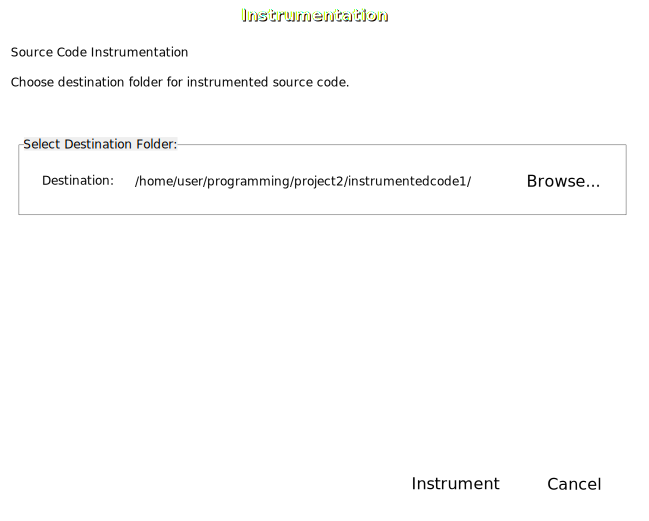
\includegraphics[width=\textwidth]{images/Instrumentation_Dialog/Instrumentation_Dialog}
 \caption{Instrumentation dialog}
 \label{ui_fg:Instrumentation dialog}
\end{figure}

\subsection{Launching} \label{ui:Launching}
The software adds a new launch mode to the Eclipse workbench. This mode is called Coverage mode and works exactly like the existing Run and Debug modes. Figure \ref{ui_fg:Coverage button} shows the pull down menu of the \eclui{Coverage Button} on the tool bar. The menu items \eclui{Coverage History}, \eclui{Coverage As} and \eclui{Coverage\dots} are added to the \eclui{Coverage} menu.
\par
The \eclui{Coverage\dots} option opens the \eclui{Coverage} dialog which is similar to the Run dialog, except that the \eclui{Run} button in that dialog is called \eclui{Coverage}.
\begin{figure}[hbtp]
 \centering
 
\includegraphics[]{images/Coverage_Button/Coverage_Button}
 \caption{Coverage button}
 \label{ui_fg:Coverage button}
\end{figure}
\par

\subsection{Coverage view}
The coverage results are presented in the \eclui{Coverage} view. It displays the results of \gl[statement]{statement}, branch, condition and \gl[loop coverage]{loop coverage} per \gl[project]{project}, package, class (including interfaces and enums) and method. This view is shown in figure \ref{ui_fg:Coverage view}.
\begin{figure}[hbtp]
 \centering
 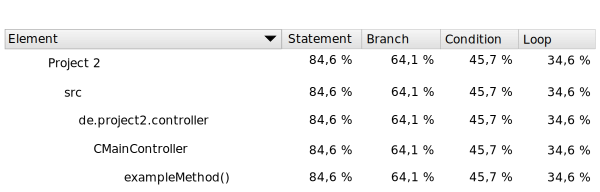
\includegraphics[]{images/Coverage_View/Coverage_View.png}
 \caption{Coverage view}
 \label{ui_fg:Coverage view}
\end{figure}
\par
A grey bar is shown left of a coverage result if there are no \gl[coverable item]{coverable items} of the associated \gl[coverage criterion]{coverage criterion} in the associated \eclui{Element}.

The check box in the upper-left corner of the view enables a simple filter if checked. If the filter is activated only methods with a coverage result smaller, smaller or equal, greater, greater or equal than a given percentage are shown in the coverage view. The coverage criterion to compare with can be selected in the most left combo box in the view. The operator to compare the coverage result with can be selected in the combo box right of the combo box of the coverage criteria. The percentage to compare with can be entered in the field right of the combo box of the comparison operators.

The tool bar items in the upper-right part of the view provide the possibility to select Java elements shown as root entries in the element column. Possible root entries are projects, packages, classes (including interfaces, enums and annotations) and methods.

\subsection{Test sessions view} \label{ui:Test sessions view}
The \eclui{Test Sessions} view lists the \gl[test session]{test sessions} of the selected \gl[session container]{session container}. Figure \ref{ui_fg:Session view} shows an example of this view. A session container can be chosen using the combo box. The session container list entries display the date and time along with the associated \gl[project]{project}.
\begin{figure}[hbtp]
 \centering
 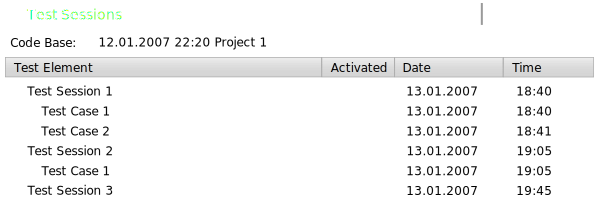
\includegraphics[]{images/Test_Case_Administration_View/Session_View.png}
 \caption{Test Sessions view}
 \label{ui_fg:Session view}
\end{figure}
\par
The check box in front of each row determines whether a \eclui{Test Element} is activated. The coverage results of activated \eclui{Test Element}s are visualized by the views of the plugin (e.g., \eclui{Coverage} view) and the source code highlighting. The visualizations are automatically refreshed as the user activates or deactivates particular \eclui{Test Element}s. By default, all \eclui{Test Element}s are activated.
\par
The activation or deactivation of a test session activates or deactivates all test cases of this test session. For test sessions the check box has an additional state, partly activated. This state is visualized by the crossed out check box in figure \ref{ui_fg:Session view} and means that at least one test case of a selected test session is deactivated. 
\par
The information about the set of active (visualized) \eclui{Test Element}s is stored; that is, selecting a new session container does not change the set of the active \eclui{Test Element}s of the previous session container.
\par
The tool bar items represent following commands (from left to right):
\begin{itemize}
\item Delete Test Session Container
  \begin{itemize}
  \item Delete Multiple Containers
  \end{itemize}
\item Merge
\item Delete
\end{itemize}
\eclui{Delete Test Session Container} deletes the active session container. Prior to the actual deletion the user has to confirm his intent to do so. By using the drop-down menu of the \eclui{Delete Session Container} item, the user can reveal the item for the deletion of multiple session containers: \eclui{Delete Multiple Containers}. It opens a dialog that prompts the user to select the session containers to delete and performs the deletion after the user confirmed the selection.  The item \eclui{Merge} allows the user to merge the selected test elements. On selection of this item a dialog pops up which prompts the user to select the type of test element (test cases or test sessions) to merge and prompts the user to enter a name and comment for the merged test element. Furthermore the user is able to review and change the set of test elements to merge. The \eclui{Delete} item deletes the selected test elements, whereas the user is asked for confirmation before the deletion is performed.
\par
The \eclui{Test Element}s have a context menu which contains following items:
\begin{itemize}
\item Select All
\item Activate All
\item Deactivate All
\item Delete
\item Properties
\end{itemize}
The item \eclui{Select All} selects all test elements of the active session container to be able to delete them all at once for example. \eclui{Activate All} and \eclui{Deactivate All} activate or respectively deactivate all test elements of the active session container. The item \eclui{Delete} evokes the same action as described above. The \eclui{Properties} item opens a dialog which allows the user to edit the properties of the selected \eclui{Test Element}. The \eclui{Test Case Properties} dialog is shown in figure \ref{ui_fg:Test case properties}. It is possible to change the name of the selected \eclui{Test Element}. Furthermore, a multi line comment may be entered.
\begin{figure}[hbtp]
 \centering
 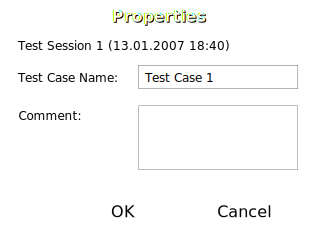
\includegraphics[width=0.5\textwidth]{images/Test_Case_Administration_View/Test_Case_Properties.png}
 \caption{Test case properties}
 \label{ui_fg:Test case properties}
\end{figure}

\subsection{Import} \label{ui:Import}
The software extends the standard Eclipse \eclui{Import} interface by adding two entries to group \eclui{\gbt}, \eclui{Test Session Container} and \eclui{\gbt Coverage Log}. Figure \ref{ui_fg:Import Test Session Container} shows the correspondent \eclui{Import} wizard page. This dialog allows the user to select a \gl[session container]{session container} and a \gl[project]{project} into which the session container will be imported. The file extensions used in the following dialogs are examples.
\begin{figure}[hbtp]
 \centering
 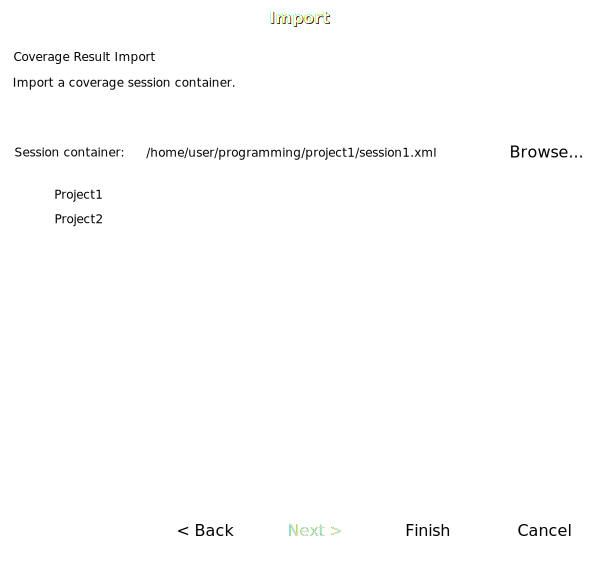
\includegraphics[width=0.85\textwidth]{images/Test_Case_Administration_View/Import_Session.png}
 \caption{Import Test Session Container}
 \label{ui_fg:Import Test Session Container}
\end{figure}
\par
Selecting \eclui{\gbt Coverage Log} proceeds with the wizard page shown in figure \ref{ui_fg:Import Coverage Log}. This import operation requires the \gl[coverage log]{coverage log} file, created while running the instrumented program. Moreover the user has to select the session container the coverage log will be imported to and enter a name and comment for the new test session that will contain the data of the coverage log.
\begin{figure}[hbtp]
 \centering
 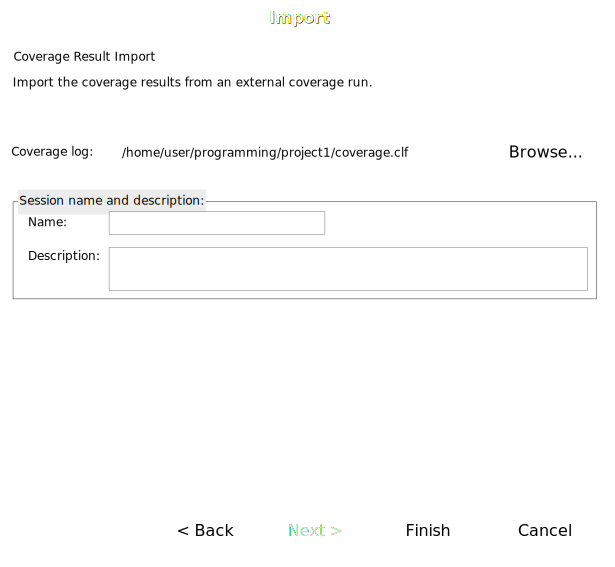
\includegraphics[width=0.9\textwidth]{images/Test_Case_Administration_View/Import_Coverage_Log.png}
 \caption{Import Coverage Log}
 \label{ui_fg:Import Coverage Log}
\end{figure}
\par

\subsection{Export} \label{ui:Export}
The item \eclui{\gbt Coverage Result Export} is added to the \eclui{Other} group of standard Eclipse \eclui{Export} dialog. The respective wizard page is shown in figure \ref{ui_fg:Export Test Session}. The dialog contains the list of all available \gl[test session]{test sessions} in the selected code base. The list \eclui{Available Test Sessions} allows multiple selections. The code base can be chosen from the combo box. By default, the last code base or the code base which is used in the \eclui{Test Sessions} view is preselected.
\begin{figure}[hbtp]
 \centering
 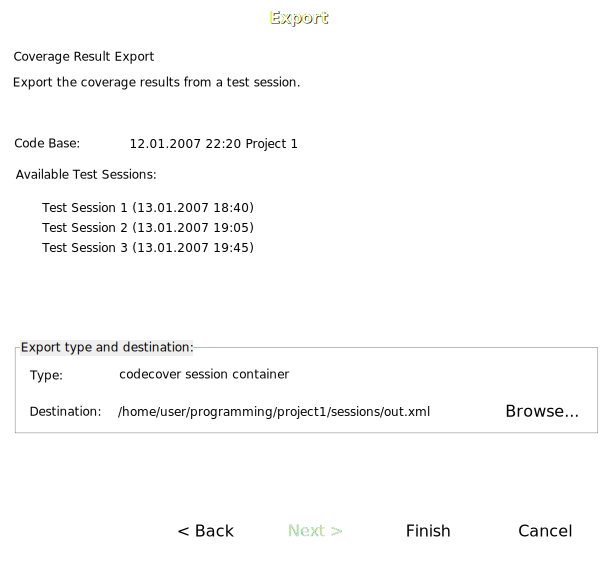
\includegraphics[]{images/Test_Case_Administration_View/Export_Session}
 \caption{Export Test Session}
 \label{ui_fg:Export Test Session}
\end{figure}
\par
Possible export types are \eclui{\gbt Session Container} and \textit{Report}. The report type has an extra wizard page which allows the user to select a report template (figure \ref{ui_fg:Report dialog}).
\begin{figure}[hbt]
 \centering
 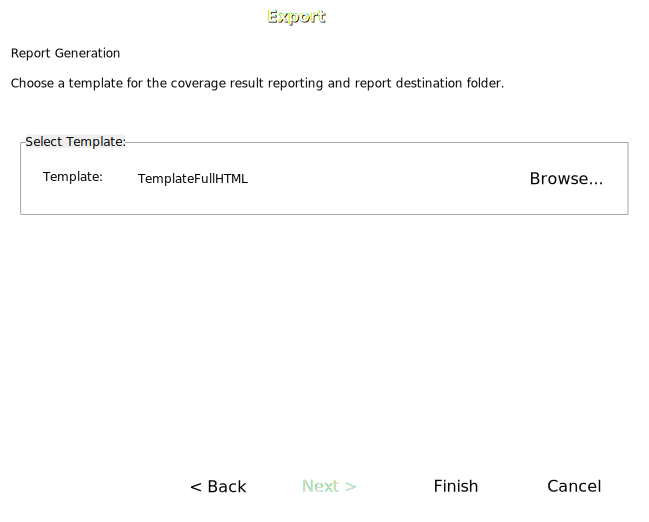
\includegraphics[width=1.0\textwidth]{images/Report_Configuration_Dialog/Report_Configuration_Dialog}
 \caption{Report dialog}
 \label{ui_fg:Report dialog}
\end{figure}
\par

\subsection{Source code highlighting} \label{ui:Source code highlighting}
\subsubsection{General}
This section describes the visualization of coverage results by highlighting  the source code of the \gl[SUT]{SUT}. There are three different colors for displaying the state of a particular part of code. The default color scheme uses green for ``covered'', yellow for ``partly covered'' and red for ``not covered''. All these colors are configurable (see section~\ref{ui:Preferences dialog}). Throughout this section, the default colors are used to explain the details of the highlighting. 

Statement coverage is shown by highlighting the \gl[statement]{statements}. To display \gl[branch coverage]{branch coverage}, the keywords of \gl[conditional statement]{conditional statements} are highlighted. Condition coverage is represented by coloring each basic term of a condition with green or red. For \gl[loop coverage]{loop coverage}, the keywords of looping statements are highlighted. All examples in this section show source code highlighting with all coverage criteria.
\subsubsection{Java}

\paragraph{Basic statements}
Basic statements are completely highlighted either green or red, for covered and not covered statements, respectively.

\paragraph{Conditional statements}
\subparagraph{If-then-else statements}
The following list describes the meaning of the background color of the \texttt{if} keyword:
\begin{itemize}
\item \textbf{Green:}  Both branches are covered.
\item \textbf{Yellow:}  Only the then-branch is covered.
\item \textbf{Red:}  Only the else-branch is covered.
\end{itemize}
\par
Figure \ref{ui_fg:If-then statements} illustrates the different possibilities of if-then coverage. If the branching statement is not evaluated because it is not executed, it is also highlighted with red color.
\begin{figure}[hbt]
 \hfill
 
\includegraphics[]{images/Source_Code_Highlighting/if/if_without_else_green}
 \hfill
 \includegraphics[]{images/Source_Code_Highlighting/if/if_without_else_yellow}
 \hfill
 \includegraphics[]{images/Source_Code_Highlighting/if/if_without_else_red}
 \hspace{1cm}
 \hfill
 \caption{If-then statements}
 \label{ui_fg:If-then statements}
\end{figure}
\par
The background color of \texttt{else} keyword has the following meanings:
\begin{itemize}
\item \textbf{Green:}  The else-branch is covered.
\item \textbf{Red:}  The else-branch is not covered.
\end{itemize}
\par
\begin{figure}[hbt]
 \hfill
 \includegraphics[]{images/Source_Code_Highlighting/if/if_with_else_green}
 \hfill
 \includegraphics[]{images/Source_Code_Highlighting/if/if_with_else_yellow}
 \hfill
 \includegraphics[]{images/Source_Code_Highlighting/if/if_with_else_red-green}
 \hspace{1cm}
 \hfill
 \caption{If-then-else statements}
 \label{ui_fg:If-then-else statements}
\end{figure}
\par
Example highlighting of if-then-else statements is shown in the figure  \ref{ui_fg:If-then-else statements}. The left picture represents full statement, branch and \gl[condition coverage]{condition coverage}. In the middle picture only the then-branch and in the right one only the else-branch is covered. 
\par
An if-then-else statement can be nested in another if-then-else statement. In that case the same color scheme as described above is applied. Figure \ref{ui_fg:Nested if-then-else statements} shows some examples for nested if-then-else statements.
\begin{figure}[htp]
 \hfill
 \includegraphics[]{images/Source_Code_Highlighting/if/if_with_else_if_green-yellow}
 \hfill
 \includegraphics[]{images/Source_Code_Highlighting/if/if_with_else_if_red-green-red}
 \hfill
 \includegraphics[]{images/Source_Code_Highlighting/if/if_with_else_if_yellow}
 \hfill
 \caption{Nested if-then-else statements}
 \label{ui_fg:Nested if-then-else statements}
\end{figure}
\par

\subparagraph{Switch statements}
The following list describes the highlighting scheme for the \texttt{switch} keyword:
\begin{itemize}
\item \textbf{Green:}  All cases are covered.
\item \textbf{Yellow:}  Some cases are covered, but at least one case is not covered.
\item \textbf{Red:}  No case is covered.
\end{itemize}
If the default section of the \texttt{switch} statement is not covered the \texttt{switch} keyword is highlighted as partly covered (yellow) as well. The highlighting is independent from the fact that the default section can be omitted. Figure \ref{ui_fg:Switch-statement with some cases and default section} shows a sample highlighted \texttt{switch} statement with a \texttt{default} section.
\par
For every case the keyword \texttt{case} and the \texttt{constant} are highlighted the following:
\begin{itemize}
\item \textbf{Green:}  The case is covered.
\item \textbf{Red:}  The case is not covered.
\end{itemize}
If the default section is not omitted, the keyword \texttt{default} is highlighted the same way as cases.

\begin{figure}[hbt]
 \centering
 \includegraphics[]{images/Source_Code_Highlighting/switch/switch}
 \caption{Switch-statement with some cases and a default section}
 \label{ui_fg:Switch-statement with some cases and default section}
\end{figure}
\par
\par

\paragraph{Looping statements}
\subparagraph{General}
The keywords of looping statements (\texttt{while}, \texttt{for} and \texttt{do-while}) are highlighted as specified in the following list. The \gl[loop coverage]{loop coverage} is defined in section \ref{fr:Loop coverage}.
\begin{itemize}
\item \textbf{Green:}  Loop body is covered (fulfill all requirements of loop coverage). 
\item \textbf{Yellow:}  Loop body is partly covered (at least one requirement of loop coverage, but not all requirements).
\item \textbf{Red:}  Loop body is not covered at all.
\end{itemize}
\par

\subparagraph{While loops}
Figure \ref{ui_fg:While statements} shows full, partly and not covered \texttt{while} loops (from left to right).
\begin{figure}[hbt]
 \hfill
 \includegraphics[]{images/Source_Code_Highlighting/while/while_green}
 \hfill
 \includegraphics[]{images/Source_Code_Highlighting/while/while_yellow}
 \hfill
 \includegraphics[]{images/Source_Code_Highlighting/while/while_red}
 \hfill
 \caption{Highlighting of while loops}
 \label{ui_fg:While statements}
\end{figure}
\par

\subparagraph{Do-while}
Do-while loop is represented similar to the \texttt{while} loop; only the \texttt{while} keyword is highlighted. The colors are the same (see figure \ref{ui_fg:Do-while statements}).
\begin{figure}[hbt]
 \hfill
 \includegraphics[]{images/Source_Code_Highlighting/do-while/do-while_green}
 \hfill
 \includegraphics[]{images/Source_Code_Highlighting/do-while/do-while_yellow}
 \hspace{2cm}
 \caption{Do-while statements}
 \label{ui_fg:Do-while statements}
\end{figure}
\par

\subparagraph{For}
The coverage results of \texttt{for} loops are visualized in the same way as those for \texttt{while} loops. Samples of highlighted \texttt{for} loops are shown in the figure \ref{ui_fg:For statements}.
\begin{figure}[hbt]
 \hfill
 \includegraphics[]{images/Source_Code_Highlighting/for/for_green}
 \hfill
 \includegraphics[]{images/Source_Code_Highlighting/for/for_yellow}
 \hfill
 \newline
 \centering
 \includegraphics[]{images/Source_Code_Highlighting/for/for_red}
 \caption{For statements}
 \label{ui_fg:For statements}
\end{figure}
\par

\subsubsection{COBOL}
\paragraph{Basic statements}
Basic statements like \texttt{DISPLAY}, \texttt{ACCEPT} or \texttt{COMPUTE} are highlighted with green and red for covered and not covered statements, respectively.

\paragraph{Conditional statements}
\subparagraph{If-then-else statements}
The highlighting scheme for if-then-else statements is completely analogous to that of the corresponding statements in Java described above. Figure \ref{ui_fg:If-then statements in COBOL} shows the highlighting of an if-then statement in the COBOL programming language:
\begin{figure}[htp]
 \hfill
 
\includegraphics[]{images/Source_Code_Highlighting/if_cobol/if_without_else_green}
 \hfill
 \includegraphics[]{images/Source_Code_Highlighting/if_cobol/if_without_else_yellow}
 \hfill
 \includegraphics[]{images/Source_Code_Highlighting/if_cobol/if_without_else_red}
 \hspace{1cm}
 \hfill
 \caption{If-then statements in COBOL}
 \label{ui_fg:If-then statements in COBOL}
\end{figure}
\par

\subparagraph{Evaluate statement}
The \texttt{EVALUATE} statement is the counterpart of the Java \texttt{switch} statement. Therefore analogous highlighting rules are applied for this statement. Figure \ref{ui_fg:Evaluate statement} shows an example of the \texttt{EVALUATE} statement highlighting:
\begin{figure}[htp]
 \centering
 \includegraphics[]{images/Source_Code_Highlighting/evaluate/evaluate}
 \caption{Evaluate statement}
 \label{ui_fg:Evaluate statement}
\end{figure}
\par

\paragraph{Looping statements}
\subparagraph{Perform}
The \texttt{PERFORM} statement is overloaded and can be used as a \gl[basic statement]{basic statement} to jump to a particular paragraph (e.g. as in figure \ref{ui_fg:Evaluate statement}) as well as a loop statement. Figure \ref{ui_fg:Perform statement with test before} shows a while-equivalent statement and figure \ref{ui_fg:Perform statement with test after} a do-while-equivalent one. The highlighting rules for the while and do-while loops in Java apply accordingly. 
\begin{figure}[htp]
 \centering
 \includegraphics[]{images/Source_Code_Highlighting/perform/perform_wtb_yellow}
 \caption{Perform statement with test before}
 \label{ui_fg:Perform statement with test before}
\end{figure}
\begin{figure}[htp]
 \centering
 \includegraphics[]{images/Source_Code_Highlighting/perform/perform_wta_yellow}
 \caption{Perform statement with test after}
 \label{ui_fg:Perform statement with test after}
\end{figure}
\par

\subsection{Preferences dialog} \label{ui:Preferences dialog}
The \gbt entry in the \eclui{Preferences} dialog contains Eclipse-wide options for configuring the software. This dialog page is shown in figure \ref{ui_fg:Preferences dialog}.
\begin{figure}[hbt]
 \centering
 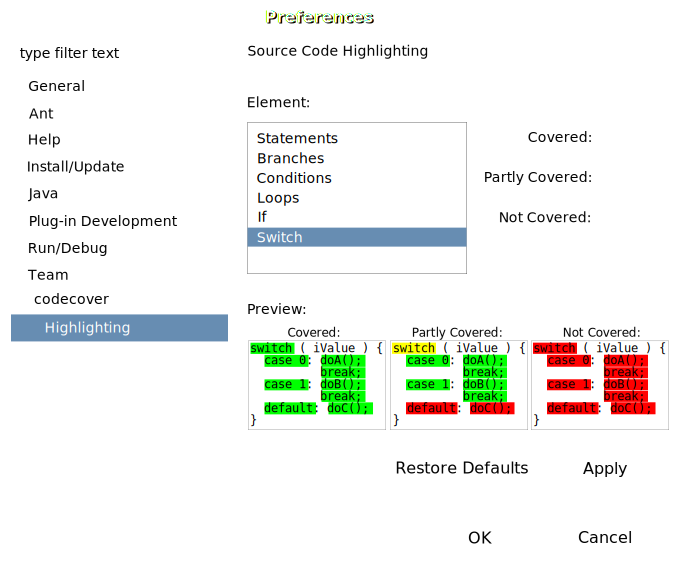
\includegraphics[width=1.0\textwidth]{images/Preferences_Highlighting/Preferences_Highlighting}
 \caption{Preferences dialog}
 \label{ui_fg:Preferences dialog}
\end{figure}
\par

\todo{adopt this fully to standard dialog for annotations. Picture may be made when it's coded.}
The dialog provides a list of annoations to configure. For each of the four metrics there are three annotations: fully covered, partly covered, not covered. For each annotation the color can be selected using the standard mechanisms of Eclipse. A partly covered state is not produced by the default metrics for basic statements, basic boolean terms and branches. However as these may very well be produced by add on metrics there are also options to configure their color.

\newpage
\subsection{Project properties dialog} \label{ui:Project properties dialog}
In the \eclui{Properties} dialog of a \gl[project]{project} a \gbt entry is added. On this page, the user can activate codecover for the project. If codecover is activated the selection of coverage criteria which are to be measured for the project is enabled too. Figure \ref{ui_fg:Project properties dialog} shows this dialog page.
\begin{figure}[hbt]
 \centering
 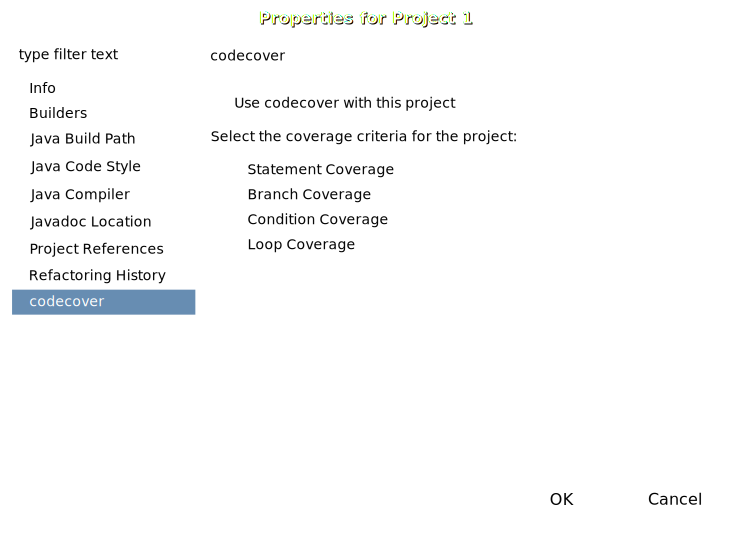
\includegraphics[width=1.0\textwidth]{images/Project_Configuration_Dialog/Project_Configuration_Dialog}
 \caption{Project properties dialog}
 \label{ui_fg:Project properties dialog}
\end{figure}

\newpage
%% \subsection{Test case notification} \label{ui:Test case notification}
%% The software extends the Eclipse menu \eclui{Source} and adds a new sub menu \eclui{\gbt Test Case Notification}. Therein new menu items are available:
%% \begin{itemize}
%%   \item \eclui{Start Test Case With Name And Comment}
%%   \item \eclui{Start Test Case With Name Only}
%%   \item \eclui{End Test Case With Name}
%%   \item \eclui{End Last Test Case}
%% \end{itemize}
%% \par
%% Also, corresponding templates are integrated to the Eclipse editor to allow easy inserting of the \gl[test case]{test case} notification statements described in section~\ref{fr:Test sessions and test cases}.

\subsection{Correlation Matrix}
\subsubsection{Mathematic prelude}\label{ui:Mathematic prelude}
The \eclui{Correlation Matrix} shows the correlation between test cases of a single test-session-container. Every test case contains a set of coverable items, which represents those parts of the code, that were covered during an execution of the instrumented system under test. Those sets are defined as follows: 
\begin{equation}
C_{T}:= \{ x | x \in T \wedge x \in CoverableItems \wedge x \in covered \}
\end{equation}

Correlation between two test cases $T_{1}$, $T_{2}$ is then defined as:
\begin{equation}
K_{U,V} := \frac{\mid U \cap V \mid}{\mid V \mid}
\end{equation}
with $U = C_{T_{1}}$ and $V = C_{T_{2}}$.
\par
Using this definition of correlation a \textit{partially ordered set} $R$ can be defined:
\begin{equation}
R = \{(U,V) \in C \times C : K_{U,V} = 1 \}
\end{equation}
In words this means, that two test cases $T_{1}$, $T_{2}$ are in relation $R$, if, and only if, $T_{1}$ contains all the coverable items $T_{2}$ does(or possibly more), which would make $T_{2}$ superfluous. This \textit{partially ordered set} then allows to detect and establish subsumption chains, in which one test cases completely contains another and so forth.
\par
Proof that $R$ is a \textit{partially ordered set} requires to proof that it possesses the following three attributes:
\begin{enumerate}
\item reflexivity
	\begin{equation}
	(U,U) \in R \Leftrightarrow \frac{\mid U \cap U \mid}{\mid U \mid} = 1 \Leftrightarrow \frac{\mid U \mid}{\mid U \mid} = 1
\end{equation}

\item antisymmetry
\begin{eqnarray}
	(U,V) \in R \Leftrightarrow \frac{\mid U \cap V \mid}{\mid V \mid} = 1 \Leftrightarrow V \subseteq U \\
	(V,U) \in R \Leftrightarrow \frac{\mid V \cap U \mid}{\mid U \mid} = 1 \Leftrightarrow U \subseteq V \\
\Rightarrow	V \subseteq U \wedge U \subseteq V \Rightarrow U = V
\end{eqnarray}

\item transitivity
\begin{eqnarray}
	(U,V) \in R \Leftrightarrow \frac{\mid U \cap V \mid}{\mid V \mid} = 1 \Leftrightarrow V \subseteq U \\
	(V,W) \in R \Leftrightarrow \frac{\mid V \cap W \mid}{\mid W \mid} = 1 \Leftrightarrow W \subseteq V \\
\Rightarrow	W \subseteq V \wedge V \subseteq U \Rightarrow W \subseteq U \Leftrightarrow \frac{\mid U \cap W \mid}{\mid W \mid} = 1 \Leftrightarrow (U,W) \in R
\end{eqnarray}

\end{enumerate}
with $T_{1}$, $T_{2}$ and $T_{3}$ being three test cases and $U = C_{T_{1}}$, $V = C_{T_{2}}$ and $W = C_{T_{3}}$.

\begin{figure}[hbt]
 \centering
 \includegraphics[width=1.0\textwidth]{images/Correlation_View/CorrelationView}
 \caption{Correlation View}
 \label{ui_fg:Correlation View}
\end{figure}
\subsubsection{Correlation View}
Using the definitions from \ref{ui:Mathematic prelude}, the view in Eclipse is defined as shown in figure~\ref{ui_fg:Correlation View}. A tree is located on the left of the view. This tree shows the subsumption chains of test cases defined in \ref{ui:Mathematic prelude}. All the children of a node in the tree are completely covered by the node itself.
\par	
The \eclui{correlation matrix} is located on the right side of the view. It shows all the test cases, that were used in the calculation of the correlation. The meaning of the colors is explained in the legend situated to the right of the matrix. The matrix is to be read from the left, e.g [test case left] covers [test case top] by [color value]\%. A tooltip shown, when hovering above one entry of the matrix, contains the exact percentage of correlation, as well as the amount of total coverable items and shared coverable items.
\par	
The tool bar items represent following commands (from left to right):
\begin{itemize}
\item Export the currently displayed matrix data into a .csv file - This command exports the data of the matrix into a comma seperated file.
\item Hide top-level tree items with no children - This command hides all the top level entries in the tree, which have no children, meaning they do not subsume any other test case;
\item Choose and calculate correlation - This command selects the metric to be used in calculating the correlation, with the pull-down menu of the arrow and calculates the correlation with a push on the button.
\item Show Legend - This command shows or hides the legend.
\item Automatically calculate correlation - If this command is toggled on, the correlation is automatically recalculated, when the selection of test case is changed. It can be switched off to improve performance.
\end{itemize}
\par
The test cases, that are to be used in the calculation, are selected using the \nameref{ui:Test sessions view}. If the \eclui{Automatically calculate correlation} command is toggled on, every change in the selection causes the correlation view to update its contents. Since this can potentially be time-consuming, the \eclui{Automatically calculate correlation} command can be toggled off and the \eclui{Choose and calculate correlation} command can be used, after the desired selection was achieved.


\subsection{Live Notification View}
\begin{figure}[hbt]
 \centering
 \includegraphics[scale=0.7]{images/Live_Notification/live_notification_view.png}
 \caption{Live Notification}
 \label{ui_fg:Live Notification}
\end{figure}
The \eclui{Live Notification View} is used to implement the \nameref{sec:fr:Live_Test_Case_Notification} (\ref{sec:fr:Live_Test_Case_Notification}). Two textfields are used to enter the hostname and port. The name of the test case can be entered as well. Test cases can be started and stopped with two labeled buttons. The test session can be finished with another button. The log file can be retrieved with the ``Download Coverage Log File'' button. This also automatically stores the data of log file in the test session container.

\subsection{Boolean Analyzer} \label{ui:Boolean Analyzer}
The \eclui{Boolean Analyzer} shows the boolean value of each basic boolean term, operator term and the root term according to evaluations of the condition which are recorded during the execution of the SUT. This data is presented in a table. The operators, operands and brackets define the columns and the evaluations are shown as rows in the table. In addition, a column for test cases is added. In that column one can see the test cases which covered the evaluation and the number of execution. 

Two table values of a column may contain green background. This represents that the basic boolean term of that column is covered according to the strict condition coverage criterion. If a column of a basic boolean term does not contain any colored values then the term is not covered. Figure \ref{ui_fg:Boolean Analyzer} shows the \eclui{Boolean Analyzer}.

\begin{figure}[hbt]
 \centering
 \includegraphics[width=1.0\textwidth]{images/Boolean_Analyzer/Boolean_Analyzer}
 \caption{Boolean Analyzer}
 \label{ui_fg:Boolean Analyzer}
\end{figure}

There are two ways to select a condition in the \eclui{Boolean Analyzer}. First, there are combo-boxes for classes and conditions. The second way is to select the keyword of the condition in the source code, right-click, and select the "Analyze Term" item in the context menu, which will automatically select the condition in the Boolean Analyzer.

\subsection{Hot-Path}\label{ui:Hot-Path}
The plugin displays line-wise execution counters corresponding to the currently selected test cases. The measured number of executions of lines is added to the \eclui{vertical ruler} of the java text editor via annotations with a color code. When the cursor hovers over such a Hot-Path annotation a tooltip with the execution counter is shown.

If no basic statement is found in a line, then no color is shown for that line in the ruler. Otherwise the color corresponding to the most often executed basic statement of that line is shown.

The color code is a mapping from the execution count of one line ($e$) and the highest exection count within a source file ($e_{max}$) to the color to mark that line. It must be encapsulated in a single method to make it easy to change in the source code. The mapping is a linear blending between the colors given in the users preferences. The exect mapping is: $color(e, e_{max}) = color_{max} * (e/e_{max}) + color_{null}(1-e/e_{max})$.

%%% Local Variables: 
%%% mode: latex
%%% TeX-PDF-mode: t
%%% TeX-master: "Specification.tex"
%%% End: 

\svnid{$Id: NonFunctionalRequirements.tex 1 2007-12-12 17:37:26Z t-scheller $}
\section{Non-functional requirements} \label{nf:Non-functional requirements}
\subsection{Technologies and development environment}
The following software is used for development:
\begin{itemize}
\item Java 5 SE
\item Eclipse 3.3.x
\item the customer's COBOL-85 grammar \footnote{bruessel.informatik.uni-stuttgart.de:/home/export/bruessel/projects/stupro06/grammars/cobol.jj}
\item Subversion 1.3.0 on the server for configuration management
\item ArgoUML 0.22 for use case diagrams in the \gl[specification]{specification}
\item BOUML 2.21.5 or compatible for UML diagrams

\end{itemize}
\par
The following technologies are used for development:
\begin{itemize}
\item LaTeX as document format
\item UTF-8 for encoding text
\item XML as the intermediate format for reports
\item Java and COBOL-85 example programs
\end{itemize}

\subsection{Requirements to the working environment}
\subsubsection{Software requirements}
%requirements to the hard- and software at the users computer
%JUnit not required but optional: JUnit for JUnit integration ~> no need to mention
The following programs are required to use the software:
\begin{itemize}
\item Java version 5 or later
\item Eclipse 3.3.x for all GUI functions
\item \gl[PDF]{PDF} viewer for documentation which supports at least PDF 1.4
%TODO: which version of JUnit? ; Iteration 3
\item JUnit for automatic \gl[test case]{test case} recognition
\item for COBOL support a COBOL-85 preprocessor to prepare code for \gl[instrumentation]{instrumentation} and a compiler to compile the instrumented code
\end{itemize}

\subsubsection{Hardware requirements} \label{nf:Hardware requirements}
%NOTE: customer mentioned no clear requirements: basically we may assert recent hardware
To support a wide installation base moderate hardware should be enough for using the software. Exact minimum requirements must be determined based on the final application.
\par
The minimum hardware required is:
\begin{itemize}
\item 512 MiB \footnote{1 MiB = $2^{20}$ Bytes} of RAM
\item a CPU as powerful as an AMD Athlon with 1 GHz clock rate
\item 100 MiB of free hard disk space for installation with Eclipse already installed, to store working data and for some \gl[session container]{session containers}
\end{itemize}

The following hardware is recommended:
\begin{itemize}
%min 512 MiB is suggested for eclipse
\item 1 GiB of RAM
%min 1 GHz is suggested for eclipse
\item a CPU as powerful as single core AMD Athlon with 2 GHz clock rate
%normally not mentioned, recent single drives achive 90 MB/s
%Johannes has ~250MB/s at home if necessary, only with 1.6GHz CPU however. 60MB/s via NFS and a fast dual core CPU could be made available
\item 60 MiB/s read and write sequential transfer rate measured at file system level
%would make ~1000 bytes per LOC when analyzing 5 Mio LOC
\item 10 GiB of free hard disk space to store working data and some coverage results
\end{itemize}

\subsection{Quantity requirements} \label{nf:Quantity requirements}
Quantities that have no defined maximum are only limited by the resources of the PC the software runs on.

\subsubsection{Program examples}
\paragraph{Small program} \label{nf:Small program}
\linkwithfootnote{http://sourceforge.net/projects/fred}{Fred v1.3.5 RC2} is a small program. All functions of the software that dont' work with it are completely useless.
\paragraph{Medium program} \label{nf:Medium program}
\linkwithfootnote{http://tomcat.apache.org/download-55.cgi}{Tomcat 5.5.20} is a medium sized program. All functions of the software must work with it.
\paragraph{Large program} \label{nf:Large program}
%is newest archived Version
\linkwithfootnote{http://archive.eclipse.org/eclipse/downloads/drops/R-3.1.2-200601181600/index.php}{Eclipse SDK 3.1.2} is a large program. Running functions on the large program is sufficient to show that they work for any \gl[project]{project} that must be supported.

\subsubsection{Timestamp}
Timestamps have a resolution of one minute or finer. The software must use a state of the art representation of timestamps to support a sufficiently wide time period.

\subsubsection{Text value}
Text values are of arbitrary length and may contain any Unicode characters.

\subsubsection{Test case}
The name and the comment of a \gl[test case]{test case} are text values. The start time is a time stamp.

\subsubsection{Test session}
An arbitrary number of \gl[test session]{test sessions} must be supported.
\par
The name and the comment of a \gl[test session]{test session} are text values. The start time is a time stamp.

\subsubsection{Code Base}
An arbitrary number of \gl[code base]{code bases} must be supported. The date and time of the first instrumentation is a time stamp.

\subsection{Performance requirements} \label{nf:Performance requirements}
All performance requirements must be met on the recommended hardware.

\subsubsection{Batch processing}
Building and instrumenting a large program (\ref{nf:Large program}) must be possible within 10 hours.

\subsubsection{Eclipse plug-in}
The following constraints must hold true for a medium program (\ref{nf:Medium program}) and should hold true for a large program (\ref{nf:Large program}).
\par
The Eclipse plug-in may not slow down Eclipse significantly.
\par
Additionally the following response times must be met. They don't apply to the first call of a function. During the first call initialization routines may add a significant delay.
\par
For simple GUI interaction 0.1 s response time is enough while 0.5 s is too slow. Selecting instrumentable items is such a simple GUI interaction.
\par
For interaction resulting in complicated rebuilds of the UI components the code highlighting 5 s response time is enough while 30 s is too slow. During this time the Eclipse UI may not respond. An example for such interaction is changing the source code annotations while they are displayed.
\par
For loading and saving files as well as processing tasks like building the correlation matrix and generating a report there are no performance requirements. These tasks may not block the Eclipse UI.

\subsection{Availability}
There are no special availability requirements.

\subsection{Security}
There are no special security requirements.

\subsection{Robustness and failure behavior} \label{nf:Robustness and failure behavior}
%how reacts the software if the puts in wrong inputs,
%e.g. a string in a date field
%what happens if Prof. Ludewig takes a seat on the keyboard
File types are detected using a syntax check for plain text files and at least 64 bit long magic numbers for binary files. That syntax check only has to detect wrong file types.
\par
The software may show arbitrary behavior when it runs on broken hardware.
%does not crash if input file is too big but shows errormessage; could be too difficult to catch any Memory Exception; TODO: Really required?

\subsection{Usability} \label{nf:Usability}
Any string displayed by the Eclipse plug-in is localizable. The default language is English.
\par
A \gl[developer]{developer} can install the software easily. The installation procedure may only require unzip and Java. The software must be installable within 5 minutes by a developer after he has found the installation instructions and downloaded the necessary files. %eases testing and spreading of the software
\par
All colors used for highlighting can be changed by the user.
\par
Internal procedures must be invisible to the user as long as he doesn't want to change their behavior. Where applicable sensible defaults must be preset.
\par
An English user's manual is required. Online help is not required.
\par
The user interface must be intuitive to the point that on line help is not needed. \linkwithfootnote{http://www.eclipse.org/articles/Article-UI-Guidelines/Index.html}{Eclipse User Interface Guidelines version 2.1} must be followed for the Eclipse plug-in. Additionally per default the user is asked in a confirm dialog before a file with valuable user data is deleted or overwritten. 
% Such dialogs have a checkbox to remember the answer permanently and not show the dialog again.
%"valuable user data" - exact enough?- example would be a session container

\subsection{Portability}
The software must run on all platforms Eclipse 3.2.x runs on.
\par
The delivered \gl[instrumentation]{instrumentation} procedure must be compatible with Java 2 version 1.4.x and Java 5 as well as preprocessed COBOL-85. Other languages must be implementable without changing the \gl[session container]{session container's} format.
\subsection{Maintainability}
The source code follows a style guide based on Sun's
\linkwithfootnote{http://java.sun.com/docs/codeconv/}{Code Conventions}. The
style guide is described in a separate document. 
\par
All technical documents made specifically for creating and verifying the software are released to the public.

\subsection{Extensibility} \label{nf:Extensibility}
The software is written to be highly extensible and documented on a level easy to understand for their target audience. The documentation of the Eclipse plug-in is written for the Eclipse user, the documentation of the batch interface is written for the shell user (see Actors \ref{fr:Actors}) and the documentation to extending the Software is written for \gl[maintenance engineer]{maintenance engineers}. Tutorials for maintenance engineers will show how to extend the software to other programming languages than COBOL and Java, how to add the collecting of metrics during the \gl[instrumentation]{instrumentation} and how to implement further coverage criteria. The tutorials may assume good knowledge of Java, Grammars, JavaCC and the languages that must be supported by the changed software.
\par
Reports can be customized using templates, which can be selected in Eclipse using a wizard. It must be easy to add new report formats like \gl[PDF]{PDF} and \gl[DocBook XML]{DocBook XML}, which can be transformed into many formats.
\par
To ease external analysis and report generation all data of a \gl[test session]{test session}, except for the boolean values sampled in \gl[conditional statement]{conditional statements}, must be available to easily implement an export to XML. The design team must decide if the \gl[session container]{session container} already has such a format, or if report generation already contains it as an intermediate step.
\par
Other coverage criteria should be easy to add for \gl[maintenance engineer]{maintenance engineers} as long as they
don't depend on execution order. No change to the \gl[instrumentation]{instrumentation}, test case management and highlighting may be necessary to implement another condition coverage criterion.
\par
%boolean and coverage analyzer, hot path visualisation and a correlation matrix
It must be easy to add further analysis of a session container. All evaluation results of boolean expressions and counters must be easily accessible.
\par
Based on the TestCaseNotifier class (see \ref{fr:Test sessions and test cases}), functions to define test cases must be added: a live mode with a graphical dialog which allows the user to start and stop test cases during the \gl[SUT]{SUT} execution and automatic test case recognition of JUnit test cases.


% --- List of figures --- %

\newpage
% \phantomsection is needed for correct PDF link to the LOF
% (see Bug 2)
\phantomsection
\listoffigures
% \addcontentsline{toc}{section}{List of figures}

% --- Glossary --- %

\newpage
\printglossary
% \addcontentsline{toc}{section}{Glossary}

\end{document}

%%% Local Variables:
%%% TeX-PDF-mode: t
%%% End: